% !TeX root = ../../main.tex

\subsection{工具总体结构设计}
\label{kebianjingguaguan}
GGQ95型可变径套管刮管器（图纸型号BJG700000A，7\inch 可变径刮壁器）是一种可通过 7\inch 套管、仅在 9-5/8\inch 套管内张开的液压可变径刮管工具：其刮刀收回外径为 136\,mm、工具本体最大外径为 139.5\,mm，均小于 7\inch 套管的内径（随磅级约为 $150\sim162$\,mm），因此下井及通过 7\inch 套管时刮刀始终收回、与井壁不接触，7\inch 套管的刮管由同趟管柱中位于本工具下方的常规 7\inch 刮管器完成；待管柱上提至 9-5/8\inch 套管井段并投球憋压激活后，刮刀方可张开（自由张开外径 229\,mm 以上，实际受 9-5/8\inch 套管内径约束贴壁），清除 9-5/8\inch 套管内壁上的残余水泥、泥块、轧制过程中产生的毛刺与鳞片、管内防砂射孔时形成的射孔飞边、生产井套管上的铁锈与水垢以及硬石蜡等影响正常施工作业的杂物；本工具与常规 7\inch 刮管器组合，实现"一趟钻完成 7\inch 与 9-5/8\inch 套管刮管"。其井身结构与管柱组合为：7\inch 套管内刮刀收回、以低于 150\,mm 的外径通过，9-5/8\inch 段投球憋压后刮刀张开贴壁，与同趟管柱下部的常规 7\inch 刮管器配合，一趟完成两级套管的刮管。其结构如图~\ref{fig:variable_scrapter_structure}所示，可变径套管刮削器由上接头、旋转连杆座、连杆、刮刀、心轴、复位总成、工作活塞、工作弹簧、下接头、节流喷嘴、中间外筒、中间心轴、激活球座、钢球以及标准件、密封件等零件组成。刮刀采用两组 5 瓣圆周错位排布，覆盖 9-5/8\inch 套管内径圆周 360° 方向。

该工具的工作原理为：下井及通过 7\inch 套管时，球座由圆周 $4\times\phi 4.80$ 剪钉定位于上位，将活塞腔与工具水眼流道隔断，刮刀由复位弹簧保持在收回位（收回外径 136\,mm），工具处于\textbf{收回待命状态}，此时可正常循环、旋转并传递扭矩与提拉、下放载荷，球未落座时泵压再高刮刀也不会张开；投球后钢球坐封球座、憋压剪断剪钉，球座下移并建立活塞腔与工具水眼流道，水眼内的液压力经工具底部节流喷嘴形成的工作压差推动工作活塞并迫使工作弹簧上行，在连杆机构的作用下刮刀张开、贴紧 9-5/8\inch 套管内壁；随后上提、下放管柱即可实现刮刀对套管内壁的刮削清洁，停泵后节流压差消失、刮刀由复位弹簧收回。工具激活为一次性、不可逆过程（图纸明细栏中不设复位球），因此 7\inch 套管的全部作业必须在投球激活之前完成。工具的上下接头分别连接管柱，并通过心轴连接，可传递扭矩和提拉、下放载荷；旋转连杆座可迫使整组刮刀绕工具自由旋转，当套管内壁变形或通过性较差时，刮刀可绕工具旋转错位通过。该工具的三个工作状态见表~\ref{tab:ggq95_states}，技术参数见表~\ref{tab:ggq95}\footnote{注：本体最大外径按图纸BJG700000A--可变径刮壁器总装图标注的$\phi 139.50$取139.50\,mm；总长按总装图标注的$2959.61\pm 2.50\,\text{mm}$取2959.61\,mm；水眼为工具最小过流内径，取图纸BJG700004A--刮刀心轴内孔$\phi 38.10$；接头扣按总装图NC38（API 7-2）标注。}。

此外，本工具上的刮刀结构与本体结构非固连，前者可绕管柱结构自由旋转。现有的刮管器刮刀与管柱大多采用固连结构，当管柱产生旋转时，刮刀也随之旋转。若套管内壁存在局部变形或通过性较差的井段，刮刀在旋转过程中可能会卡住，而刮刀的杆系机构承受侧向载荷的能力很差，极有可能导致杆系机构卡死，引起卡钻事故。本工具设置了两组端面及周向回转机构，滚道中的填充的了滚珠，形成了滚动摩擦副，刮刀可绕管柱自由旋转，避免了刮刀卡死的风险。

\begin{table}[htbp]
    \centering
    \caption{可变径刮管器工作状态}
    \label{tab:ggq95_states}
    \footnotesize
    \setlength{\tabcolsep}{4pt}
    \renewcommand{\arraystretch}{1.3}
    \begin{tabular}{p{2.4cm}p{2.6cm}p{2.2cm}p{2.6cm}p{3.4cm}}
        \toprule
        工作状态 & 球座位置 & 剪钉与活塞腔 & 刮刀外径 & 可进行的作业 \\
        \midrule
        收回待命（投球前） & 上位，隔断活塞腔与水眼流道 & 剪钉完好、完好隔断 & 136\,mm（本体 139.5\,mm） & 循环、旋转、传递扭矩、通过 7\inch 套管，由下部常规 7\inch 刮管器完成 7\inch 段刮管及其它作业 \\
        激活（投球憋压） & 剪钉剪断、球座下移，不可逆 & 流道建立、活塞腔连通 & 由 136\,mm 开始张开 & 出现"泵压先升后突降"的激活特征 \\
        张开刮削（激活后循环） & 下位（永久） & 连通，节流工作压差 $\le 4$\,MPa & 张开贴壁（自由张开 229\,mm 以上） & 上提、下放刮削 9-5/8\inch 套管 \\
        停泵（激活后） & 下位（永久） & 连通但无压差 & 复位弹簧收回至 136\,mm & 起钻，通过内径较小的井段 \\
        \bottomrule
    \end{tabular}
\end{table}

\begin{figure}[htbp]
	\centering
	\includegraphics[width=1.\textwidth]{figure/chapter3/part5/variable-scrapter-structure.png}
	\caption{可变径刮管器结构示意图}
	\label{fig:variable_scrapter_structure}
\end{figure}

\begin{table}[htbp]
    \centering
    \caption{GGQ95型可变径套管刮管器技术参数}
    \label{tab:ggq95}
    \renewcommand{\arraystretch}{1.2} % 适当增加行高，提升阅读体验
    \small % 调整整体字号，适应表格宽度
    \begin{tabular}{ccccccc}
        \toprule
        型号 & \begin{tabular}[c]{@{}c@{}}本体最大外径\\(mm)\end{tabular} & \begin{tabular}[c]{@{}c@{}}刮刀收回最小外径\\(mm)\end{tabular} & \begin{tabular}[c]{@{}c@{}}刮刀最大外径\\(mm)\end{tabular} & \begin{tabular}[c]{@{}c@{}}水眼\\(mm)\end{tabular} & \begin{tabular}[c]{@{}c@{}}总长\\(mm)\end{tabular} & \begin{tabular}[c]{@{}c@{}}接头扣\\(API)\end{tabular} \\
        \midrule
        GGQ95 & 139.50 & 136 & 229+ & 38.1 & 2959.61 & NC38 \\
        \bottomrule
    \end{tabular}
\end{table}



\subsection[可变径刮管工具设计计算与校核]{可变径刮管工具设计计算与校核\protect\footnote{合同条款：5.2.1.3井筒高效清洁关键技术配套工具设计——（4）可变径刮管工具：抗拉$>=100\mathrm{T}$，抗扭$>17\,\mathrm{kN}\cdot\mathrm{m}$}}


\subsubsection{主要受力件的螺纹强度校核}

9-5/8\inch 可变径刮壁器的主要受力件为刮刀心轴，其主要受力螺纹为 $\mathrm{Tr}\,65 \times 4-8e$，危险截面即位于该螺纹的根部。

螺纹牙的剪切强度按下式计算：
\begin{equation}
	\begin{aligned}
	    F_{\max} &= [\tau] \cdot k_z \cdot \pi \cdot d_1 \cdot b \cdot z \cdot 10^{-3} \\
	    [\tau] &= \frac{\sigma_{\mathrm{s}}}{n}
	\end{aligned}
	\end{equation}
	
式中，$F_{\max}$--工具最大拉力，kN（设计指标 $\ge 1000$\,kN，见本节脚注所列合同条款 5.2.1.3（4）：抗拉 $\ge 100$\,T）；

$[\tau]$--螺纹牙的许用剪切强度，MPa（按 $[\tau]=\sigma_{\mathrm{s}}/n$ 计算）；

$k_z$--螺纹各圈的载荷不均系数，取 $k_z = 0.56$（按《机械设计手册》螺纹连接（紧固件连接）部分中螺纹牙的剪切强度计算及各圈螺纹载荷分配的规定\cite{ref26}）；

$d_1$--螺纹底径，取 62\,mm（图号 BJG700004A--刮刀心轴主视图：左端标注 $\mathrm{Tr}\,68\times4-8e$、右端标注 $\mathrm{Tr}\,65\times4-8e$ 梯形外螺纹，标准 GB/T 5796，按牙型高度换算取小径 62\,mm）；

$b$--螺纹牙根宽度，取 $b = 2.6\,\text{mm}$（按 GB/T 5796 规定的梯形螺纹牙型，由螺距 $p=4\,\text{mm}$ 与牙型高度计算）；

$z$--旋合圈数，取 $z = 23.5$（图号 BJG700004A--刮刀心轴主视图：左端螺纹旋合长度标注 94\,mm，除以螺距 4\,mm 得 23.5 圈）；

$\sigma_{\mathrm{s}}$--材料最小屈服强度，取 1068\,MPa（图号 BJG700004A--刮刀心轴技术要求第 1 条：调质后屈服强度 $\ge 1068$\,MPa、抗拉强度 $\ge 1138$\,MPa、延伸率 $\ge 12\%$；材料 4330V）；

$n$--安全系数，取 $n = 2.5$（按《机械设计手册》螺纹连接部分中螺纹牙强度校核的安全系数取值规定\cite{ref26}）。

将 $\mathrm{Tr}\,65 \times 4-8e$ 螺纹的相关参数代入，计算得：
\begin{equation}
    \begin{aligned}
    F_{\max} &= [\tau] \cdot k_z \cdot \pi \cdot d_1 \cdot b \cdot z \cdot 10^{-3} \\
             &= 427.2 \times 0.56 \times 3.14 \times 62 \times 2.6 \times 23.5 \times 10^{-3} \\
             &= 2845.65\,\mathrm{kN} \\
             &> 1000\,\mathrm{kN}
    \end{aligned}
\end{equation}
计算结果表明，螺纹牙的剪切强度满足设计要求。


\subsubsection{主要受力件的零件抗拉强度校核}

9-5/8\inch 可变径刮壁器的主要受力件为刮刀心轴和心轴连接筒，两者的抗拉危险截面分别为刮刀心轴小螺纹 $\mathrm{Tr}\,65 \times 4-8e$ 螺纹根部和心轴连接筒内螺纹 $\mathrm{Tr}\,65 \times 4-8H$ 螺纹根部。

抗拉强度按下式计算：
\begin{equation}
    F_{\max} = \frac{\pi \cdot (D^2 - d^2) \cdot \sigma_{\mathrm{s}}}{4 \cdot n} \times 10^{-3}
\end{equation}
式中，$F_{\max}$--工具最大拉力，kN（设计指标 $\ge 1000$\,kN，见本节脚注所列合同条款 5.2.1.3（4）：抗拉 $\ge 100$\,T）；

$D$--危险截面外径，mm（刮刀心轴取 62\,mm：图号 BJG700004A--刮刀心轴主视图右端牙槽根外圆标注 $\phi 58^{-0.03}_{-0.048}$，与 $\mathrm{Tr}\,65\times4-8e$ 螺纹底径取 62\,mm；心轴连接筒取 80\,mm：图号 BJG700014A--心轴连接筒主视图外圆标注 $\phi 80^{-0.03}_{-0.06}$）；

$d$--危险截面内径，mm（刮刀心轴取 38.1\,mm，依据图号 BJG700004A--刮刀心轴主视图内孔标注 $\phi 38.10$，即工具水眼；心轴连接筒取 62.2\,mm，依据图号 BJG700014A--心轴连接筒局部视图标注 $\phi 62.20^{+0.07}_0$）；

$\sigma_{\mathrm{s}}$--材料最小屈服强度，取 1068\,MPa（图号 BJG700004A--刮刀心轴技术要求第 1 条：调质后屈服强度 $\ge 1068$\,MPa、抗拉强度 $\ge 1138$\,MPa；心轴连接筒按同一材料等级取值），另按 $\phi 80/\phi 66$ 截面复核时危险截面内径取 $66\ \mathrm{mm}$；依据Tr65$\times$4梯形内螺纹（GB/T 5796）的牙根直径基本值$65.5\ \mathrm{mm}$，考虑牙底公差上限后，偏安全取整为66 mm用于强度校核。（图号 BJG700014A 内孔标注）；


$n$--安全系数，取 $n = 1.5$（按《机械设计手册》机械零部件强度计算中安全系数的取值规定\cite{ref26}）。

（1）刮刀心轴危险截面最大抗拉计算
\begin{equation}
    \begin{aligned}
    F_{\max} &= \frac{\pi \cdot (D^2 - d^2) \cdot \sigma_{\mathrm{s}}}{4 \cdot n} \times 10^{-3}
             = \frac{3.14 \times (62^2 - 38.1^2) \times 1068}{4 \times 1.5} \times 10^{-3} \\
             &= 1337.15\,\mathrm{kN} > 1000\,\mathrm{kN}
    \end{aligned}
\end{equation}
满足设计要求。

按图样退刀槽最小直径 $\phi 58.05$ 复核时，净截面面积为 $1506.6\,\mathrm{mm^{2}}$，许用拉力为 $1072.7\,\mathrm{kN}$，仍大于 $1000\,\mathrm{kN}$；$1000\,\mathrm{kN}$ 拉力下的名义拉应力为 $663.8\,\mathrm{MPa}$，对应安全系数为 $1.61$，同样满足 1.5 的判据。该截面的有限元评定应力为 $658.9\,\mathrm{MPa}$（见表~\ref{tab:fatigue_var}），与解析值基本一致。

（2）心轴连接筒危险截面最大抗拉计算
\begin{equation}
    \begin{aligned}
    F_{\max} &= \frac{\pi \cdot (D^2 - d^2) \cdot \sigma_{\mathrm{s}}}{4 \cdot n} \times 10^{-3}
             = \frac{3.14 \times (80^2 - 66^2) \times 1068}{4 \times 1.5} \times 10^{-3} \\
             &= 1142.43\,\mathrm{kN} > 1000\,\mathrm{kN}
    \end{aligned}
\end{equation}
满足设计要求。

需要说明的是，心轴连接筒的危险截面应取内螺纹 $\mathrm{Tr}\,65\times4-8H$ 根部（小径 $\phi 62.20$，见图BJG700014A），此时
\begin{equation}
    \begin{aligned}
    F_{\max} &= \frac{3.14 \times (80^2 - 62.2^2) \times 1068}{4 \times 1.5} \times 10^{-3}
             = 1414.72\,\mathrm{kN} > 1000\,\mathrm{kN}
    \end{aligned}
\end{equation}
亦满足设计要求。按图纸BJG700014A的技术要求，该件材料为 4330V（屈服强度$\ge 1068$\,MPa，抗拉强度$\ge 1180$\,MPa，硬度$341\sim401$\,HB），与刮刀心轴同一材料等级，故上述两个截面的许用拉力分别为 $1142.43\,\mathrm{kN}$（$\phi 80/\phi 66$）与 $1414.72\,\mathrm{kN}$（$\phi 80/\phi 62.2$）；在 $1000\,\mathrm{kN}$ 轴向拉力作用下，两截面的名义拉应力分别为 $623.2\,\mathrm{MPa}$ 与 $503.3\,\mathrm{MPa}$，对应 $1068\,\mathrm{MPa}$ 屈服强度的安全系数分别为 $1.71$ 与 $2.12$，均大于设计要求的 1.5。


\subsubsection{主要受力件的零件抗扭强度校核}\label{sec:torsion-var}

9-5/8\inch 可变径刮壁器的主要受力件为刮刀心轴和心轴连接筒，其抗扭危险截面与抗拉校核相同，分别位于刮刀心轴小螺纹 $\mathrm{Tr}\,65 \times 4-8e$ 螺纹根部和心轴连接筒内螺纹 $\mathrm{Tr}\,65 \times 4-8\mathrm{H}$ 螺纹根部。

抗扭强度按下式计算：
\begin{equation}
    \begin{aligned}
        \tau &= \frac{16 \cdot D \cdot T_{\max}}{\pi \cdot (D^4 - d^4)} \times 10^{6} \\
        T_{\max} &= \frac{[\tau] \cdot \pi \cdot (D^4 - d^4)}{16 \cdot D} \times 10^{-6} \\
        [\tau] &= n \cdot \sigma_{\mathrm{s}} = 0.66 \times 1068\,\mathrm{MPa} = 704.88\,\mathrm{MPa}
    \end{aligned}
\end{equation}
式中，$T_{\max}$--工具最大扭矩，kN$\cdot$m（设计指标 $>17$\,kN$\cdot$m，见本节脚注所列合同条款 5.2.1.3（4））；

$\tau$--危险截面的切应力，MPa（按 $\tau = 16DT_{\max}/[\pi(D^4-d^4)]$ 计算）；

$[\tau]$--材料许用切应力，MPa（按 $[\tau]=n\sigma_{\mathrm{s}} = 0.66\sigma_{\mathrm{s}}$ 计算）；

$\sigma_{\mathrm{s}}$--材料屈服强度，取 1068\,MPa（图号 BJG700004A--刮刀心轴技术要求第 1 条：调质后屈服强度 $\ge 1068$\,MPa）；

$D$--危险截面外径，mm（取值与抗拉校核相同：刮刀心轴 $D = 62$\,mm，图号 BJG700004A 左端牙槽根外圆；心轴连接筒 $D = 80$\,mm，图号 BJG700014A 外圆标注 $\phi 80\,{-0.03}/{-0.06}$）；

$d$--危险截面内径，mm（取值与抗拉校核相同：刮刀心轴 $d = 38.1$\,mm，图号 BJG700004A 内孔 $\phi 38.10$；心轴连接筒 $d = 66$\,mm，依据Tr65$\times$4梯形内螺纹（GB/T 5796）的牙根直径基本值$65.5\ \mathrm{mm}$，考虑牙底公差上限后，偏安全取整为66 mm用于强度校核。）；

$n$--许用切应力与许用拉应力之比，取 $n = 0.66$（按《机械设计手册》零件强度校核中许用应力折减系数的取值规定\cite{ref26}；其理论依据为第四强度理论，纯剪切时 $\tau_{\mathrm{s}} = \sigma_{\mathrm{s}}/\sqrt{3} \approx 0.577\sigma_{\mathrm{s}}$，工程上取 $0.66$ 作为折减系数）。

（1）刮刀心轴危险截面最大抗扭计算
\begin{equation}
    \begin{aligned}
    T_{\max} &= \frac{[\tau] \cdot \pi \cdot (D^4 - d^4)}{16 \cdot D} \times 10^{-6}
             = \frac{704.88 \times 3.14 \times (62^4 - 38.1^4)}{16 \times 62} \times 10^{-6} \\
             &= 28.27\,\mathrm{kN}\cdot\mathrm{m} > 17\,\mathrm{kN}\cdot\mathrm{m}
\end{aligned}
\end{equation}
满足设计要求。

（2）心轴连接筒危险截面最大抗扭计算
\begin{equation}
    \begin{aligned}
    T_{\max} &= \frac{[\tau] \cdot \pi \cdot (D^4 - d^4)}{16 \cdot D} \times 10^{-6}
             = \frac{704.88 \times 3.14 \times (80^4 - 66^4)}{16 \times 80} \times 10^{-6} \\
             &= 38.02\,\mathrm{kN}\cdot\mathrm{m} > 17\,\mathrm{kN}\cdot\mathrm{m}
\end{aligned}
\end{equation}
满足设计要求。

（3）刮刀心轴退刀槽截面受扭复核

以上（1）（2）按 $\mathrm{Tr}\,65\times4$ 螺纹根部截面（取 $D=62$\,mm）计算，但图号 BJG700004A 右端（$\mathrm{Tr}\,65\times4-8e$ 端）在 $\phi 58\,{-0.03}/{-0.048}$ 处为螺纹退刀槽，其直径比 $\mathrm{Tr}\,65\times4$ 的外螺纹小径（$\phi 60.5$）还小 2.45\,mm，是刮刀心轴全长的最小净截面，也是受扭的实际控制截面。按本节抗扭强度公式以 $D=58.05$\,mm、$d=38.10$\,mm 复核：
\begin{equation}
    \begin{aligned}
    \tau &= \frac{16 \times 58.05 \times 17 \times 10^{6}}{\pi \times (58.05^4 - 38.10^4)} = 543.5\,\mathrm{MPa} \\
    \sigma_{\mathrm{eq}} &= \sqrt{3}\,\tau = 941.4\,\mathrm{MPa} \\
    T_{\max} &= \frac{704.88 \times 3.14 \times (58.05^4 - 38.10^4)}{16 \times 58.05} \times 10^{-6} = 22.05\,\mathrm{kN}\cdot\mathrm{m}
    \end{aligned}
\end{equation}
按本章 $[\tau]=0.66\sigma_{\mathrm{s}}$ 的许用切应力口径，$17\,\mathrm{kN}\cdot\mathrm{m}$ 下的剪应力 543.5\,MPa 小于许用值 704.88\,MPa，抗扭能力 22.05\,kN$\cdot$m 大于 17\,kN$\cdot$m，按该口径仍满足要求；但 $[\tau]=0.66\sigma_{\mathrm{s}}$ 是按第三强度理论取的经验系数，比按第四强度理论（von Mises）的 $\sigma_{\mathrm{s}}/\sqrt{3}=0.577\sigma_{\mathrm{s}}$ 宽松约 14\%。按 von Mises 等效应力评定，该截面的安全系数为 $1068/941.4=1.13$，低于 1.5 的判据。需要说明的是，该式按全部扭矩经该截面传递计算，未计端面台肩接触面对扭矩的分担，结果偏保守；以 \ref{sec:fea-var} 节五件装配模型在净截面上的探针读数 627.9\,MPa 评定，安全系数为 1.70，满足 1.5 的判据，详见下文（3）。若按解析峰值口径控制，则 $17\,\mathrm{kN}\cdot\mathrm{m}$ 下退刀槽直径应放大到 $\phi 63.5$ 以上（相当于 $\mathrm{Tr}\,68\times4$ 的小径，该端螺纹须同步放大），此时等效应力降至 673\,MPa、安全系数 1.59；或把额定扭矩限制在 $12.9\,\mathrm{kN}\cdot\mathrm{m}$ 以内。


\subsubsection{球座剪钉剪切力与节流泵压计算}

9-5/8\inch 可变径刮壁器需要投球后憋压将球座剪钉剪断，迫使球座下移建立压力通道才能开始工作，因此剪钉的剪断力和投球后球座处的憋压压力是激活工具的重要参数。

刮壁器的球座圆周设计 4 组剪钉参与剪切（图纸BJG700015A--球座标注 $4\times 4.80\,{+0.20}/0$ 剪钉孔），剪钉选用 45 号非调质料制作，则工具激活所需的推力为：
\begin{equation}
    \begin{aligned}
        F_s \ge [\tau] \cdot A = 0.6 \times [\sigma] \times 4 \times (\pi \cdot R^2) &= 0.6 \times 450 \times 4 \times 3.14 \times 2.4^2 \\
        &= 19534.4\,\mathrm{N}
    \end{aligned}
\end{equation}
式中，$F_s$--工具激活所需的最小推力，N（按 $F_s = [\tau]A$ 计算，需大于剪钉总剪切力的设计值）；

$[\tau]$--材料许用剪应力，MPa（塑性材料取 $0.6[\sigma]$、脆性材料取 $0.8[\sigma]$；45 号钢为塑性材料，故按 $0.6[\sigma]$ 取值，即 $0.6\times450 = 270\,\mathrm{MPa}$）；

$[\sigma]$--材料许用拉应力，取 450\,MPa（剪钉材料为 45 号非调质钢，按 GB/T 699 中 45 钢的强度指标取值）；

$A$--参与剪切的剪钉总剪切面积，mm$^2$（$A = n_s \cdot \pi R^2$，剪钉数量 $n_s = 4$，按图号 BJG700015A--球座端面标注的 $4\times 4.80\,{+0.20}/0$ 剪钉孔均布）；

$R$--单个剪钉的半径，mm（图号 BJG700015A--球座端面剪钉孔径标注 $4.80^{+0.20}_0$，取 $R = 2.4$\,mm）。

刮壁器投入钢球后球座流道被堵塞，井口泵压直接作用在球座上，根据上述计算所得的最小推力 $F_s$，可计算出激活工具所需的最小泵压 $P_0$：
\begin{equation}
    P_0 \ge \frac{F_s}{A_q} = \frac{F_s}{\pi \cdot \left(\frac{d}{2}\right)^2} = \frac{19534.4}{3.14 \times \left(\frac{40.08}{2}\right)^2} = 15.48\,\mathrm{MPa}
\end{equation}
式中，$P_0$--激活工具所需的最小泵压，MPa（按 $P_0 = F_s/A_q$ 计算，$F_s$ 取上式所得 19534.4\,N）；

$A_q$--球座承压面积，mm$^2$（$A_q = \pi (d/2)^2$，按球座锥面所受泵压投影面积计算）；

$d$--球座承压面直径，mm（取 40.08\,mm，图号 BJG700015A--球座主视图标注的球座锥面大径）。

计算表明，当泵压不小于 $15.48\,\mathrm{MPa}$ 时，工具可以被激活。若按脆性材料系数 $0.8[\sigma]$ 偏安全计算，则 $F_s = 26045.9\,\mathrm{N}$，对应最小泵压为 $20.65\,\mathrm{MPa}$，两种取值下激活泵压均在常规作业泵压范围内。


\subsubsection{节流喷嘴的尺寸和节流压力关系}

刮壁器激活后流道建立，工具底部的节流喷嘴形成的节流压差为工具提供工作压力 $\Delta P \le 4\,\mathrm{MPa}$，故需要计算节流喷嘴的尺寸与节流压力的关系。

由公式：
\begin{equation}
    \Delta P \le \frac{827 \cdot \rho \cdot Q^2}{C^2 \cdot d_e^4}
\end{equation}

推算喷嘴最小直径为：
\begin{equation}
    d_e \ge \sqrt[4]{\frac{827 \cdot \rho \cdot Q^2}{C^2 \cdot \Delta P}} = \sqrt[4]{\frac{827 \times 1.1 \times 40^2}{0.96^2 \times 4}} = 25.06\,\mathrm{mm}
\end{equation}
式中，$d_e$--喷嘴节流孔最小直径，mm（取 25\,mm，图号 BJG700023A--$\phi 25$ 节流喷嘴主视图标注节流孔 $\phi 25$，材料 YG6，装于工具底部）；

$\Delta P$--刮壁器最大节流压力（即最大节流工作压差），MPa（按工具设计要求取 $\Delta P \le 4$\,MPa）；

$\rho$--钻井液密度，g/cm$^3$（取 $1.1$\,g/cm$^3$，按现场常用钻井液密度取值）；

$Q$--工作时泵排量，L/s（暂定取 $40$\,L/s，按常规洗井排量取值）；

$C$--流量系数，无因次，取 $0.95 \sim 0.98$，本文计算取 $C = 0.96$（按孔口流量公式的常规定值）；

$827$--工程单位制换算系数。该式由孔口流量公式 $Q = C \cdot A \cdot \sqrt{2\Delta P/\rho}$ 换算而来：将 $\Delta P = \dfrac{8\rho Q^2}{\pi^2 C^2 d_e^4}$ 中的密度取 g/cm$^3$、排量取 L/s、直径取 mm、压差取 MPa，则系数为 $\dfrac{8\times 10^{9}}{\pi^2\times 10^{6}} = 810.6$。本文取$827$，相当于流量系数 $C$ 取 $0.945$，与所取 $C = 0.95\sim0.98$ 的下限基本一致，偏安全。

按图纸BJG700023A--Φ25节流喷嘴，节流喷嘴内孔为 $\phi 25$（材料 YG6），即取 $d_e = 25\,\mathrm{mm}$。反向校核：当 $d_e = 25\,\mathrm{mm}$、$C = 0.96$、$Q = 40\,\mathrm{L/s}$ 时，
\begin{equation}
    \Delta P = \frac{827 \times 1.1 \times 40^2}{0.96^2 \times 25^4} = 4.04\,\mathrm{MPa}
\end{equation}
与设计工作压差 $\Delta P \le 4\,\mathrm{MPa}$ 基本一致；若取 $C = 0.97$，则 $\Delta P = 3.95\,\mathrm{MPa} \le 4\,\mathrm{MPa}$，满足设计要求。


\subsubsection{连杆销抗剪切强度计算}

9-5/8\inch 可变径刮壁器在激活后的工作过程中，刮壁作业所承受的冲击载荷由连杆铰链销承受，故有必要计算连杆销的抗剪切强度。假定刮壁器作业时受到的最大轴向力为工具最大抗拉力，即 $F_{\max} = 1000\,\mathrm{kN}$；销钉材料按图纸BJG700005A--活动座铰链销、BJG700007A刮刀铰链销的技术要求选用 4145H，$[\sigma] \ge 760\,\mathrm{MPa}$；销钉设计最小直径为：

由切应力公式
\begin{equation}
    \tau = \frac{F_{\max}}{A} = \frac{F_{\max}}{40 \cdot A_0} = \frac{F_{\max}}{\pi \cdot 40 \cdot \left(\frac{d}{2}\right)^2} \le [\tau]
\end{equation}
式中，$[\tau]$--材料许用剪应力，MPa（塑性材料取 $0.6[\sigma]$、脆性材料取 $0.8[\sigma]$；4145H 为塑性材料，故取 $[\tau] = 0.6 \times 760 = 456\,\mathrm{MPa}$，其中 $[\sigma] \ge 760$\,MPa 取自图号 BJG700005A--活动座铰链销、BJG700007A--刮刀铰链销技术要求第 1 条）；

$A$--参与剪切的连杆销总剪切面积，mm$^2$（每个连杆销有两个剪切面积，单个销的剪切面积为 $2A_0$；按图号 BJG700000A--可变径刮壁器总装图，刮刀共 10 把（BJG700006A 59BPF 刮刀，数量 10），每把由 2 个刮刀铰链销（BJG700007A，共 20 个）与 2 个活动座铰链销（BJG700005A，共 20 个）铰接，则单向承载的销数为 20 个，总剪切面积 $A = 2A_0 \times 20 = 40A_0$）；

$d$--连杆销的最小直径，mm（取 10\,mm，图号 BJG700005A--活动座铰链销、BJG700007A--刮刀铰链销主视图标注铰链销直径均为 $\phi 10\,{-0.04}/0$）。

可得
\begin{equation}
    d \ge 2\sqrt{\frac{F_{\max}}{40 \cdot \pi \cdot [\tau]}} = 2\sqrt{\frac{1.0 \times 10^{6}}{40 \times 3.14 \times 456}} = 8.35\,\mathrm{mm}
\end{equation}

设计连杆销直径 $d = 10\,\mathrm{mm}$（图纸BJG700005A--活动座铰链销、BJG700007A），大于计算所需的最小直径，满足设计要求。按所选 $\phi 10$ 销复核剪应力：
\begin{equation}
    \tau = \frac{1.0 \times 10^{6}}{40 \times \frac{3.14 \times 10^{2}}{4}} = 318.3\,\mathrm{MPa} < [\tau] = 456\,\mathrm{MPa}
\end{equation}
对应材料屈服强度的安全系数为 $760/318.3 = 2.39$，大于设计要求的 1.5。


\subsubsection{主要受力件仿真校核}\label{sec:fea-var}

主要受力件为刮刀心轴和心轴连接筒，危险截面出现在螺纹根部及变径处。计算材料取本节前述材料参数（屈服强度 1068\,MPa），按安全系数 1.5 计，材料许用拉应力为 712\,MPa、许用切应力为 704.88\,MPa。由于有限元模型对螺纹段作了简化、未建立螺纹牙及螺纹根部，螺纹根部的强度由前述理论公式校核，有限元计算用于复核零件本体段的应力水平，计算结果如图~\ref{fig:FEA_inner_pipe_variable}所示。

（1）刮刀心轴受拉。按工具实际装配的传力方式施加约束与载荷：刮刀心轴两端均为螺纹连接，在一端螺纹连接部位施加 1000\,kN（\(1.0\times10^{6}\)\,N）轴向拉力，另一端螺纹连接部位约束轴向位移，使零件径向可自由收缩。计算结果表明，最大等效应力（von Mises）为 1307\,MPa，出现在刮刀槽之间的变径凸台处；该处应力沿轴向迅速衰减，变径附近的等效应力为 485.9\,MPa，远离变径区的等效应力仅为 113.4\,MPa，表明高应力区局限于凸台根部很小的范围内，属变径处几何突变引起的局部应力集中，不会引起整体塑性变形。以 485.9\,MPa 作为评定值，小于材料许用拉应力 712\,MPa，对应材料屈服强度 1068\,MPa 的安全系数为 2.20，大于设计要求的 1.5；同时施加的拉力小于该零件按理论校核所得许用拉力 1337.15\,kN，故刮刀心轴的抗拉强度满足设计要求。

（2）刮刀心轴受扭。同样按工具实际装配的传力方式施加约束与载荷：在一端螺纹连接部位施加 17\,kN$\cdot$m 扭矩，另一端螺纹连接部位约束周向位移。计算结果表明，最大等效应力（von Mises）为 244.2\,MPa，出现在约束端附近的台阶处，零件本体段的等效应力为 $120\sim195$\,MPa，应力分布平稳，未出现局部奇异峰值。最大等效应力小于材料许用切应力 704.88\,MPa，对应材料屈服强度 1068\,MPa 的安全系数为 4.37，大于设计要求的 1.5；同时施加的扭矩小于该零件按理论校核所得许用扭矩 28.27\,kN$\cdot$m，故单件模型下刮刀心轴的抗扭强度满足设计要求。需要指出的是，该单件模型未建立 $\phi 58$ 退刀槽，实际控制截面并未参与计算，而 $17\,\mathrm{kN}\cdot\mathrm{m}$ 在该截面上即可产生 543\,MPa 的剪应力，故上述结果只反映螺纹段与本体段的应力水平，抗扭强度的最终评定见下文（3）。

（3）五件装配模型受扭复核。前述单件模型未建立退刀槽，结果不能代表实际控制截面，为此按工具实际装配关系建立上接头、两件刮刀心轴、心轴连接筒与下接头的五件装配模型，螺纹副与端面台肩按绑定接触处理，下端面全约束，上端面几何中心设远程点并施加 $17\,\mathrm{kN}\cdot\mathrm{m}$ 扭矩，绕轴线方向的转动自由、径向位移与另两个转动自由度约束。计算结果表明，全场最大等效应力为 1832\,MPa，出现在刮刀心轴 $\phi 58$ 退刀槽牙槽根与键合面交界的凹角处；该处为几何奇异点，应力随网格加密不收敛，不作为评定值。扭矩经该处螺纹退刀槽传递，其净截面为 $\phi 58.05/\phi 38.10$（$1506.5\,\mathrm{mm}^2$）。在该净截面上取三处探针（节点 28326、28018、28155），等效应力读数分别为 621.17、627.85、625.37\,MPa，三者相对差 1.1\%，取最大值 627.9\,MPa 作为评定值。该值与按同一截面薄壁圆轴解析计算的 $\tau=543.4$\,MPa、von Mises 941\,MPa 相差 33\%，原因是解析式按全部扭矩经该截面传递、未计端面台肩接触面的分担，偏保守；两者的结论一致——控制截面是退刀槽而非螺纹牙。以 627.9\,MPa 评定，静强度安全系数为 $1068/627.9=1.70$。扭转按完全反向（$R=-1$，覆盖正反转、倒划眼与憋钻释放等换向情形）取定载荷谱，$\sigma_a=627.9$\,MPa、$\sigma_m=0$，无需 Goodman 折算，由 4330V-1068 的 S-N 关系（$\sigma_a=5337N^{-0.2337}$）反算寿命 $9.5\times10^{3}$ 次，200 趟累积损伤 0.021（裕度约 47 倍），疲劳安全系数 $1062/627.9=1.69$。需说明的是，ANSYS 疲劳模块的设定为应力寿命、平均应力理论取 Goodman、疲劳强度因子 $K_f=1$、应力分量取带符号的 von Mises；载荷谱按完全反向（$R=-1$）施加，以覆盖正反转与憋钻释放等换向情形，此时 $\sigma_m=0$，Goodman 折算不改变应力幅，故云图与本节按 $R=-1$ 换算的寿命、损伤同源：探针节点处的寿命读数为 $1.37\times10^{4}$ 次，较换算值 $9.5\times10^{3}$ 次高约四成，属节点解与云图积分点插值之差，评定取较低的换算值。各项均高于判据，可变径刮管工具在 $17\,\mathrm{kN}\cdot\mathrm{m}$ 额定扭矩下的抗扭强度满足要求，控制部位为刮刀心轴的 $\phi 58$ 退刀槽，结果见表~\ref{tab:torsion_var}。

尚需说明的是，距奇异点约 3\,mm 的凹角邻域峰值为 921\,MPa，应力集中系数约 1.47（921/627.9），对应静强度安全系数 1.16、疲劳安全系数 1.15，低于 1.5 的判据；该值是圆角为零的尖角模型在几何突变处形成的局部峰值，只在有限元中随网格加密而增大。加工时应保证退刀槽与 $\phi 68$ 台肩过渡处的圆角不小于 R1，并在总装后复算；若圆角无法保证，则应按该峰值口径把额定扭矩限制在 $12.9\,\mathrm{kN}\cdot\mathrm{m}$ 以内，或把退刀槽净截面放大到 $\phi 63.5$ 以上（该端 $\mathrm{Tr}\,65\times4$ 螺纹须同步放大为 $\mathrm{Tr}\,68\times4$，此时等效应力降至 673\,MPa、安全系数 1.59）。另需指出，本模型只建五个主体零件、未计外筒 BJG700013A 传扭，扭矩全部由芯轴链承担，计算结果偏保守。

\begin{table}[htbp]
\centering
\caption{可变径刮管工具扭转工况有限元复核结果}
\label{tab:torsion_var}
\begin{tabular}{lcc}
\hline
项目 & 数值 & 判据 \\
\hline
全场最大等效应力 / MPa & 1832（凹角奇异，不评定） & --- \\
凹角邻域峰值应力 / MPa & 921（不计入评定） & --- \\
评定应力 / MPa & 627.9（净截面探针） & --- \\
静强度安全系数 & 1.70 & $\ge 1.5$ \\
计算寿命 / 次 & $9.5\times10^{3}$ & --- \\
200 次累积损伤 & 0.021 & $\le 1.0$ \\
疲劳安全系数 & 1.69 & $\ge 1.5$ \\
\hline
\end{tabular}
\end{table}

\begin{figure}[htbp]
	\centering
	\subfloat[可变径刮管器心轴]{%
	\includegraphics[width=0.7\textwidth]{figure/chapter3/part5/inner-pipe.png}
	}
	\hfill
	\subfloat[抗拉强度分析]{%
	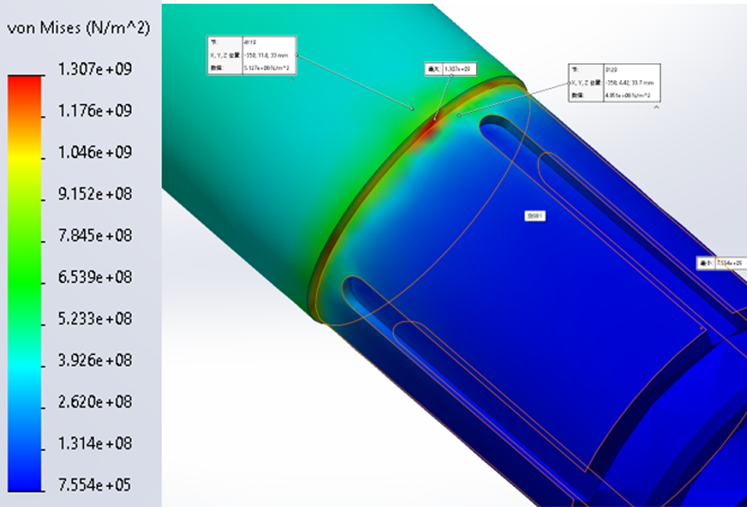
\includegraphics[width=0.45\textwidth]{figure/simulation/guadaoxinzhou-lashen.png}
	}
	\vspace{1em}
	\subfloat[抗扭强度分析]{%
	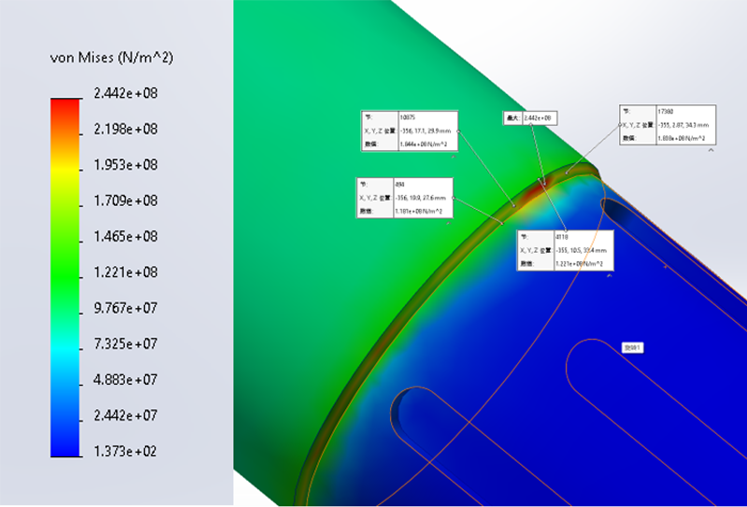
\includegraphics[width=0.45\textwidth]{figure/simulation/gaudaoxinzhou-niuju.png}
	}
	\caption{可变径刮管工具薄弱零件强度有限元分析}
	\label{fig:FEA_inner_pipe_variable}
\end{figure}



\begin{figure}[htbp]
	\centering
	\subfloat[左段]{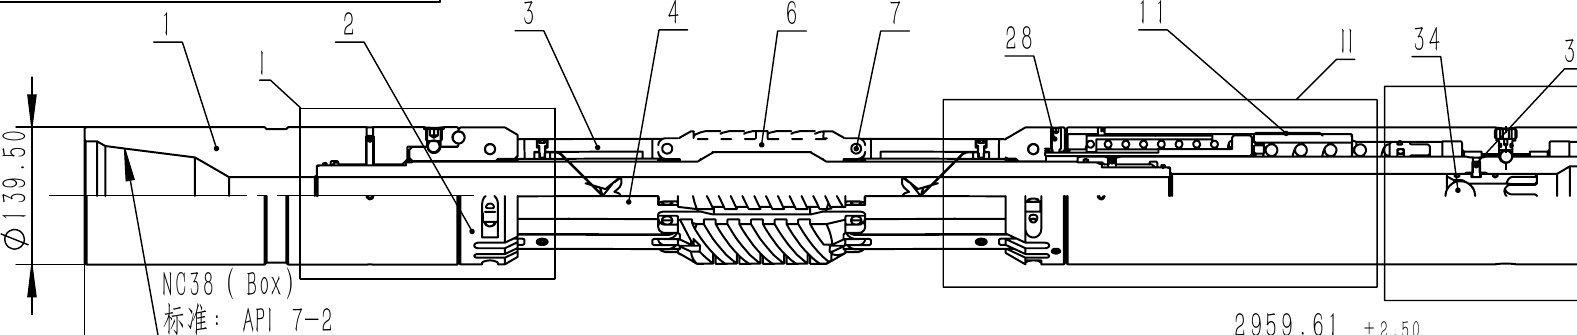
\includegraphics[width=\textwidth]{figure/chapter3/dwg-ggq-a.png}}\\[2pt]
	\subfloat[右段]{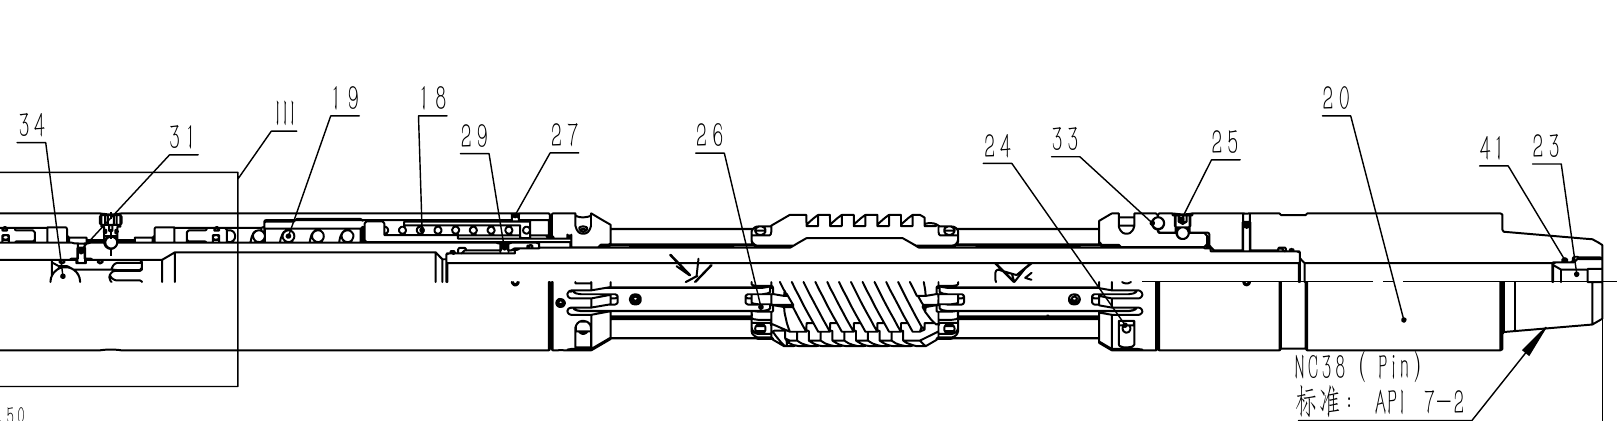
\includegraphics[width=\textwidth]{figure/chapter3/dwg-ggq-b.png}}
	\caption{BJG700000A 可变径刮管器二维总装图（纵剖主视图，比例 1:8）}
	\label{fig:dwg-ggq}
\end{figure}

\subsection{适用井况与作业场景}

本工具适用于 9-5/8\inch 套管内壁清洁作业场景，需在通过 7\inch 套管后方可进入目标层段开展工作，
主要用于清除套管内壁残余水泥、泥块、轧制毛刺、鳞片、防砂射孔残留弹片、铁锈、水垢、硬石蜡等影响
施工作业的附着物。

适用作业场景包括新井射孔前通井（保障完井工具顺利下入及封隔器座封）与老井维护修井（清除套管内壁
附着物、恢复井筒通畅度）。工具需与 7\inch 及以上规格其它刮管器配合使用，并根据井况选配适配的节流
喷嘴及剪钉，以满足不同泵压与排量的工艺要求。

\subsection{管柱组合}

可变径刮管器应作为钻柱的一个功能段进行串接，推荐自上而下组合为：上部钻柱 $+$（选装其它套管清洁
工具）$+$ 可变径刮管器 $+$ 7\inch 刮管器 $+$ 与套管规格对应的扶正器 $+$ 通井钻头。可变径刮管器
上接头经 NC38 与上部管柱连接，下接头与下部 7\inch 刮管器或加重短节连接。

入井前须确认刮刀处于收回状态：本体最大外径 139.50\,mm、刮刀收回后 136\,mm（见表~\ref{tab:ggq95}），
可顺利通过 7\inch 套管（最小内径约 150\,mm）后进入 9-5/8\inch 套管目标作业层位。管柱组合应遵循
“前端配扶正器、与 7\inch 刮管器协同作业”的原则，所有连接螺纹必须按规范扭矩上紧，确保刮管作业
过程中扭矩与提拉力的有效传递。

\subsection{施工工艺步骤}

\subsubsection{下井前准备}
\begin{itemize}
	\item 了解井况，确定套管规格和深度等基本信息；
	\item 选配适合套管规格的刮刀；
	\item 本可变径刮管器应与 7\inch 及以上其它刮管器配合使用；本工具刮刀收回外径 136\,mm、本体最大外径 139.5\,mm，在 7\inch 套管内与井壁不接触，7\inch 套管的刮管应由同趟管柱中位于本工具下方的常规 7\inch 刮管器完成；
	\item 确定刮管工艺，了解泵压和排量，并根据图~\ref{fig:pressure_decrease_with_Q_size}所示不同排量下喷嘴尺寸与压降的关系选装合适的喷嘴及剪钉。
\end{itemize}

\begin{figure}[htbp]
	\centering
	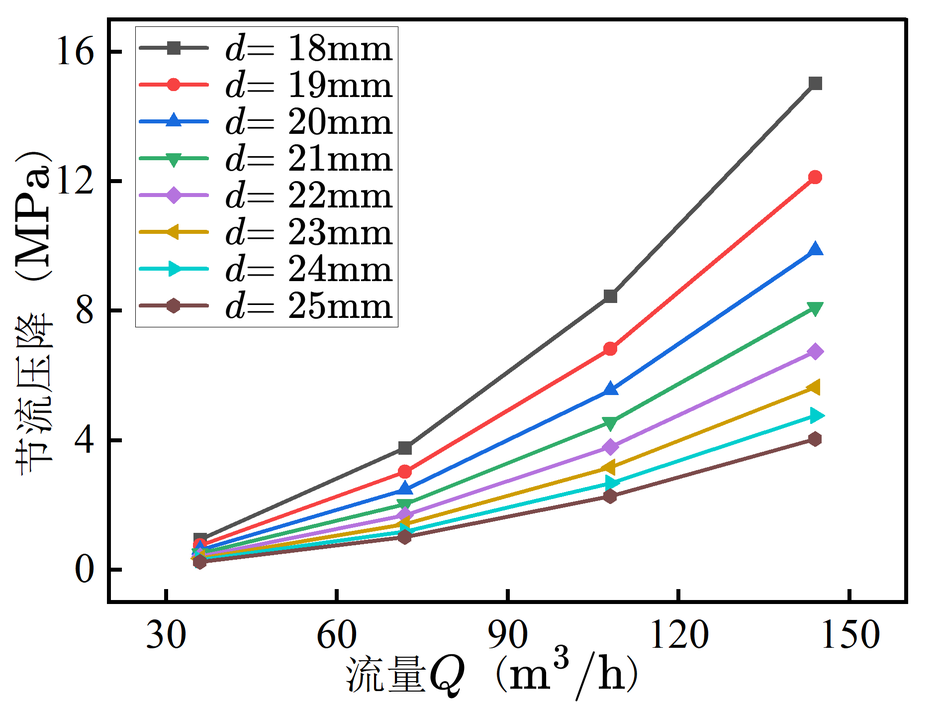
\includegraphics[width=0.5\textwidth]{figure/chapter3/3-3.png}
	\caption{喷嘴压降与排量、喷嘴尺寸之间的关系}
	\label{fig:pressure_decrease_with_Q_size}
\end{figure}


\subsubsection{作业顺序}
可变径刮管器的完整作业顺序为"先小规格套管、后 9-5/8\inch 套管；投球一次、激活不可逆"：随管柱下入时刮刀收于刀槽内（收回外径 136\,mm），在 7\inch 套管内以收回状态通过，小规格段的刮管由管柱下部的常规 7\inch 刮管器承担；上提至 9-5/8\inch 套管井段后投球憋压，剪钉剪断、刮刀张开贴壁，自下而上刮削 9-5/8\inch 套管内壁，如图~\ref{fig:ggq95_workseq}所示。具体步骤如下：

\begin{figure}[htbp]
	\centering
	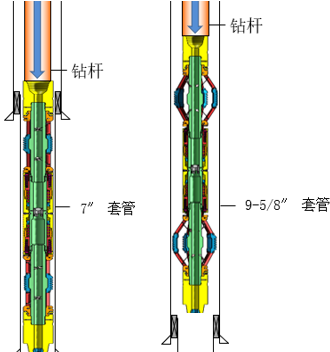
\includegraphics[width=0.55\textwidth]{figure/chapter3/part5/ggq95-workseq.png}
	\caption{可变径刮管器的工作顺序（左：在 7\inch 套管内刮刀收回、随管柱下行通过；右：上提至 9-5/8\inch 套管、投球憋压后刮刀张开贴壁刮削）}
	\label{fig:ggq95_workseq}
\end{figure}

\begin{enumerate}[label=(\arabic*),leftmargin=2em,itemsep=2pt]
	\item \textbf{入井前检查与选配}：确认套管规格与井深；检查刮刀能否自由收回至 136\,mm、球座圆周 $4\times\phi 4.80$ 剪钉是否完好；按设计排量选装节流喷嘴（标准件为 $\phi 25$ 喷嘴 BJG700023A）；备好并登记现场投球用 $\phi 30$ 钢球（图纸明细栏"钢球 30-G20"1 件）。需注意明细栏中 100 件 $\phi 12$ 钢球（钢球 12-G40）为装配用限位钢球，不是现场投球，二者不得混用。
	\item \textbf{组配管柱}：下井前按照作业要求依次连接好管柱，刮管器前端需接与套管规格对应的扶正器；推荐管柱组合为：通井钻头 $+$ 扶正器 $+$ 7\inch 刮管器 $+$ 可变径刮管器 $+$（选装其它套管清洁工具）$+$ 上部钻柱。
	\item \textbf{地面试循环}：接上可变径刮管器后，夹紧下接头、大钳打上接头，拧紧刮管器各螺纹，井口以开泵压力 $\le 20 \pm 5\,\mathrm{MPa}$、排量 $\le 10\,\mathrm{L/s}$ 进行试循环，时间 $1 \sim 5\,\mathrm{min}$；确认循环正常、各连接无刺漏，并确认刮刀未弹出本体（仍为收回状态）。此时未投球、球座未憋压，泵压不作用于球座，刮刀不会张开。
	\item \textbf{下钻}：控制下放速度，慢慢旋转下放工具；全程保持钻井液循环畅通。本工具在 9-5/8\inch 与 7\inch 套管中均为收回通过状态，不参与刮削。
	\item \textbf{7\inch 套管段作业}：在 7\inch 套管内由下部常规 7\inch 刮管器完成刮管，并进行其它钻磨、完井、试油、测试等作业。本工具此时未激活、不参与 7\inch 段刮削；7\inch 段的全部作业必须在投球激活之前完成。
	\item \textbf{上提至 9-5/8\inch 套管井段}：当小规格套管刮管及其它作业完成后，将可变径刮管器提升至 9-5/8\inch 套管所需的井深位置，确认工具已完全脱离 7\inch 段（含尾管悬挂器、回接筒等小内径部位）后，投入 $\phi 30$ 钢球，开泵打压激活刮刀张开，启动作业。
	\item \textbf{憋压激活}：刮管器打开压力 $=$ 静液柱压力 $+$ 泵压（绝对压力），即泵压 $\ge$ 绝对压力 $-$ 静液柱压力；按\ref{kebianjingguaguan}节计算，球座剪钉剪断所需的最小泵压为 $15.5\,\mathrm{MPa}$（按塑性材料系数）$\sim 20.7\,\mathrm{MPa}$（按脆性材料系数），现场应以先达到该泵压再回落作为激活判据。
	\item \textbf{激活判定}：投入钢球后观察泵压，若泵压上升过程中突然下降，说明可变径刮管器已启动；随后停泵，按工具入井前选定的喷嘴尺寸所要求的泵压和排量稳定循环，同时通过上提、下放工具进行 9-5/8\inch 套管的刮管作业。
	\item \textbf{9-5/8\inch 套管刮管}：在稳定循环（节流工作压差 $\le 4\,\mathrm{MPa}$）条件下上提、下放工具刮削；刮管作业时观察指重表无任何显示，即下放悬重不降、上提悬重不升，表明已刮削干净。
	\item \textbf{停泵、起钻}：刮管作业完成后先停泵，使节流压差消失、刮刀由复位弹簧收回至 136\,mm，再按规定的起钻速度起出管柱；起钻过程中注意悬重与摩阻变化。
	\item \textbf{出井拆检与保养}：按拆装步骤拆开清洗，更换全部 O 形圈与失效弹簧，检查球座、剪钉孔、刮刀、铰链销及密封面，并按要求保养存放。
\end{enumerate}

\subsection{拆装步骤}

工具出井后，到达管子站进行保养前，需冲洗外表面，并准备好内六角扳手、起子、扳手等拆卸工具。

(1) 工具冲洗干净后，将上、下接头的 M16 螺钉拆卸，取出内部的防掉钢珠；取出下接头喷嘴；如下图箭头所示位置。

\begin{figure}[H]
\centering
	\includegraphics[width=1.\textwidth]{figure/chapter3/part5/unsetup/ball.png}
\end{figure}

(2) 拆卸上、下接头的防松螺钉后，分别反转拆卸上、下接头；如下图所示位置。

\begin{figure}[H]
\centering
	\includegraphics[width=1.\textwidth]{figure/chapter3/part5/unsetup/unsetup-satefy-screw.png}
	\vspace{1em}
	\includegraphics[width=1.\textwidth]{figure/chapter3/part5/unsetup/unsetup-two-subs.png}
\end{figure}

(3) 用起子、扳手取下连杆座、连杆、刮刀等之间的铰链销、防掉螺钉等标准件后，依次拆卸旋转连杆座、连杆、刮刀等零件；如下图所示。

\begin{figure}[H]
\centering
	\includegraphics[width=1.\textwidth]{figure/chapter3/part5/unsetup/unsetup-fasten-parts.png}
\end{figure}

(4) 拆卸各部位的锁紧螺钉、铰链销、防掉螺钉等零件。

(5) 拆卸两头的旋转连杆座。

\begin{figure}[H]
\centering
	\includegraphics[width=1.\textwidth]{figure/chapter3/part5/unsetup/rotary-lever-set.png}
\end{figure}

(6) 拆卸两头的连杆、刮刀等零件。

\begin{figure}[H]
\centering
	\includegraphics[width=1.\textwidth]{figure/chapter3/part5/unsetup/end-links.png}
	\includegraphics[width=1.\textwidth]{figure/chapter3/part5/unsetup/unsetup-scraper.png}
	\includegraphics[width=1.\textwidth]{figure/chapter3/part5/unsetup/left-links.png}
\end{figure}

(7) 分别反转拆卸两头的心轴，从下部取出激活球座和钢球，如下图所示。

\begin{figure}[H]
\centering
	\includegraphics[width=1.\textwidth]{figure/chapter3/part5/unsetup/unsetup-inner-pipe.png}
	\includegraphics[width=1.\textwidth]{figure/chapter3/part5/unsetup/unsetup-ball-and-seat.png}
\end{figure}

(8) 夹紧中间外筒方向旋转复位总成，分别取出上、下两头的复位总成，然后依次对复位总成进行拆解，如下图所示。

\begin{figure}[H]
\centering
	\includegraphics[width=1.\textwidth]{figure/chapter3/part5/unsetup/reseting-assembly.png}
	\includegraphics[width=1.\textwidth]{figure/chapter3/part5/unsetup/resetting-assembly-unsetup.png}
\end{figure}

(9) 取出中间筒体和中间心轴的限位钢球，随后取下中间心轴、弹簧、活塞、活塞限位套等零件；最后拆卸各零件上的密封圈，即拆卸完毕。

(10) 拆卸中间筒体和中间心轴的钢球堵和限位钢球。

\begin{figure}[H]
\centering
	\includegraphics[width=1.\textwidth]{figure/chapter3/part5/unsetup/middle-body-inner-pipe-ball.png}
\end{figure}

(11) 拆卸中间心轴，固定中间筒体后从任意一头抽出中间心轴即可。

\begin{figure}[H]
\centering
	\includegraphics[width=1.\textwidth]{figure/chapter3/part5/unsetup/middle-inner-pipe-unsetup.png}
\end{figure}

(12) 按下图所示方向，分别从两头拆卸活塞、工作弹簧、活塞限位套等零件。

\begin{figure}[H]
\centering
	\includegraphics[width=1.\textwidth]{figure/chapter3/part5/unsetup/piston-spring-limiter.png}
\end{figure}

(13) 装配步骤与拆卸步骤相反，装配过程中需要注意不要损伤密封面、螺纹牙形等配合处，密封面和螺纹组装前要求涂抹润滑油。

工具的易损件及配件清单见表~\ref{tab:parts_list}。

\begin{table}[htbp]
    \centering
    \caption{易损件及配件清单表（按图纸BJG700000A--可变径刮壁器总装图明细栏）}
    \label{tab:parts_list}
    \footnotesize % 代号较长，缩小字号以适应表格宽度
    \setlength{\tabcolsep}{4pt} % 减小列间距，避免超出正文版心
    \renewcommand{\arraystretch}{1.35} % 调整行间距，使表格不拥挤
    \begin{tabular}{clllc}
        \toprule
        序号 & 代号 & 名称 & 材料 & 单套数量 \\
        \midrule
        1  & BJG700001A & 上接头 & 4145H & 1 \\
        2  & BJG700002A & 上活动连杆座 & 4145H & 2 \\
        3  & BJG700003A & 连杆 & 4145H & 20 \\
        4  & BJG700004A & 刮刀心轴 & 4330V（屈服强度$1068\,\mathrm{MPa}$） & 2 \\
        5  & BJG700005A & 活动座铰链销 & 4145H & 20 \\
        6  & BJG700006A & 59BPF刮刀 & 20CrNiMo & 10 \\
        7  & BJG700007A & 刮刀铰链销 & 4145H & 20 \\
        8  & BJG700008A & 下活动连杆座 & 4145H & 2 \\
        9  & BJG700009A & 连杆座连接筒 & 4145H & 2 \\
        10 & BJG700010A & 中间调节堵 & 4145H & 2 \\
        11 & BJG700011A & 中间限位套 & 4145H & 2 \\
        12 & BJG700012A & 中间活塞 & 4145H & 2 \\
        13 & BJG700013A & 中间筒体 & 4145H & 1 \\
        14 & BJG700014A & 心轴连接筒 & 4330V（屈服强度$1068\,\mathrm{MPa}$） & 1 \\
        15 & BJG700015A & 球座 & 4145H & 1 \\
        16 & BJG700016A & 丝堵 & 316 & 2 \\
        17 & BJG700017A & 密封堵 & 316 & 2 \\
        18 & BJG700018A & 复位弹簧 & 60Si2MnA & 2 \\
        19 & BJG700019A & 工作弹簧 & 60Si2MnA & 2 \\
        20 & BJG700020A & 下接头 & 4145H & 1 \\
        21 & BJG700021A & 支撑弹片 & 50CrVA & 20 \\
        22 & BJG700022A & 弹片压块 & 4145H & 20 \\
        23 & BJG700023A & $\phi 25$ 节流喷嘴 & YG6 & 1 \\
        24 & GB/T 77-2007 & 内六角平端紧定螺钉 M10$\times$35 & 钢 12.9级 & 20 \\
        25 & GB/T 77-2007 & 内六角平端紧定螺钉 M16$\times$12 & 钢 12.9级 & 2 \\
        26 & GB/T 80-2007 & 内六角凹端紧定螺钉 M5$\times$16 & 钢 12.9级 & 40 \\
        27 & GB/T 77-2007 & 内六角平端紧定螺钉 M8$\times$8 & 钢 12.9级 & 8 \\
        28 & GB/T 79-2007 & 内六角圆柱端紧定螺钉 M10$\times$25 & 钢 12.9级 & 10 \\
        29 & GB/T 80-2007 & 内六角凹端紧定螺钉 M8$\times$10 & 钢 12.9级 & 8 \\
        30 & GB/T 80-2007 & 内六角凹端紧定螺钉 M8$\times$30 & 钢 12.9级 & 8 \\
        31 & GB/T 77-2007 & 内六角平端紧定螺钉 M8$\times$16 & 钢 12.9级 & 10 \\
        32 & GB/T 70.1-2008 & 内六角圆柱头螺钉 M6$\times$12 & 钢 12.9级 & 20 \\
        33 & GB/T 308.1-2013 & 钢球 12-G40 & G95Cr18 & 100 \\
        34 & GB/T 308.1-2013 & 钢球 30-G20 & G95Cr18 & 1 \\
        35 & NL6 & 防松垫片 & 65Mn HRC$39\sim44$ & 20 \\
        36 & 2-143 & O 形圈 $\phi 61.6\times2.62$ & FKM90 & 2 \\
        37 & 2-140 & O 形圈 $\phi 56.82\times2.62$ & FKM90 & 2 \\
        38 & 2-147 & O 形圈 $\phi 67.95\times2.62$ & FKM90 & 2 \\
        39 & 2-222 & O 形圈 $\phi 37.69\times3.53$ & FKM90 & 2 \\
        40 & 2-243 & O 形圈 $\phi 104.37\times3.53$ & FKM90 & 2 \\
        41 & 2-223 & O 形圈 $\phi 40.87\times3.53$ & FKM90 & 1 \\
        42 & 2-110 & O 形圈 $\phi 9.19\times2.62$ & FKM90 & 2 \\
        43 & ON 0800 052 00110 D & 双作用格莱圈 & FKM90+PTFE & 2 \\
        \bottomrule
    \end{tabular}
\end{table}

\subsection{注意事项}
\begin{itemize}
	\item 工具与管柱的连接扣必须拧紧。
	\item 两组刮刀的螺旋升角应保持同方向。
	\item 可变径刮管器在下井过程中如遇阻，应慢慢旋转几圈后再下放。
	\item 刮管作业过程中，必须始终保持钻井液循环畅通。
	\item 工具激活为一次性、不可逆过程，图纸明细栏中不设复位球，因此不得在 7\inch 套管内投球激活，也不得在 7\inch 段作业尚未全部完成时投球。
	\item 激活后带泵循环时刮刀处于张开状态（自由张开外径 229\,mm 以上），禁止带泵循环、带压进入 7\inch 套管或任何内径小于刮刀张开外径的井段，以免顶死刮刀、损坏连杆与铰链销甚至造成卡钻；起钻通过小内径井段前应先停泵，并确认刮刀已收回。
	\item 刮刀张开后受套管内径约束贴壁，实际工作直径即 9-5/8\inch 套管内径；不得以盲目提高泵压的方式追求刮削效果，工作压差由节流喷嘴限定在 $4\,\mathrm{MPa}$ 以内，刮净以指重表判据为准。
\end{itemize}

\subsection{疲劳分析}
\label{sec:fatigue-var}

\subsubsection{取值}

可变径套管刮管工具的承力件分属两档材料，须建立两条 S-N 曲线。刮刀芯轴与心轴连接筒经设计方确认改用 4330V 的 1\,068/1\,180 档：$k_a=4.51\times1\,180^{-0.265}=0.692$、$k_b=0.748$、$k_c=0.85$、$k_d=1.0$、$k_e=0.814$，五项系数之积为 0.358，$S_e=0.5\times1\,180\times0.358\approx211.3$\,MPa；$1\times10^{3}$ 次处 $0.9\sigma_u=1\,062$\,MPa 尚低于屈服强度 1\,068\,MPa，无需截断，五点拟合得 $\sigma_a=5\,337\,N^{-0.2337}$，$\sigma_e=1\,062$\,MPa。上下接头仍为 4145H 的 760/965 档：$S_e=182.3$\,MPa，$0.9\sigma_u=868.5$\,MPa 超过屈服强度，按屈服截断取 760\,MPa，拟合得 $\sigma_a=3\,169\,N^{-0.2067}$。两条曲线的斜率相差 13\%，不得互换使用。

轴向拉伸工况的峰值 2\,156.6\,MPa 位于刮刀芯轴内孔变径台阶根部，属几何尖角引起的数值奇异。距该点 3$\sim$6\,mm 的探针读数 658.88\,MPa（节点 28315）与 660.2\,MPa（节点 28313）相差 0.2\%，沿轴向再远数毫米降至 277.9\,MPa（节点 28330），梯度之陡由此可见，取 658.88\,MPa 评定。该值可与解析式互证：按 $\phi58.05/\phi38.10$ 净截面（1\,506.5\,mm$^2$）反算名义应力为 663.8\,MPa，与有限元相差 0.7\%，说明模型在同一截面上给出的是可用的工程应力，而非数值假象。评定结果列于表~\ref{tab:fatigue_var}。

\begin{table}[htbp]
\centering
\caption{可变径套管刮管工具的疲劳评定结果（200 趟）}
\label{tab:fatigue_var}
\begin{tabularx}{\textwidth}{lCCC}
\hline
项目 & 轴向拉伸（$R=0$） & 抗扭（$R=-1$） & 判据 \\
\hline
额定工况 & 1\,000\,kN & 17\,kN$\cdot$m & --- \\
评定应力 / MPa & 658.88 & 921 & --- \\
应力幅与平均应力 / MPa & 329.44 & 921 / 0 & --- \\
等效对称应力幅 / MPa & 457.0 & 921 & --- \\
计算寿命 / 次 & $3.7\times10^{4}$ & $1.9\times10^{3}$ & --- \\
200 次累积损伤 & $5.4\times10^{-3}$ & 0.106 & $\le 1.0$ \\
疲劳安全系数 & 1.70 & 1.15 & $\ge 1.5$ \\
静强度安全系数 & 1.62 & 1.16 & $\ge 1.5$ \\
判定 & 满足 & 不满足 & --- \\
\hline
\end{tabularx}
\end{table}

拉伸工况的计算过程为：$\sigma_a=\sigma_m=329.44$\,MPa，$\sigma_{a,\mathrm{eq}}=329.44/(1-329.44/1\,180)=457.0$\,MPa，反解得 $N=(5\,337/457.0)^{1/0.2337}=3.7\times10^{4}$ 次，$D=200/3.7\times10^{4}=5.4\times10^{-3}$，$n_f=1/(329.44/1\,062+329.44/1\,180)=1.70$，$n_s=1\,068/658.88=1.62$，各项均在判据之内，与工具族其余三种 1\,000\,kN 级工具处于同一水平。

扭转工况的结论则不同。17\,kN$\cdot$m 下峰值 1\,832\,MPa 出现在刮刀芯轴 $\phi58$ 退刀槽根与键合面交界的凹角，属数值奇异；评定应力取退刀槽净截面上的 921\,MPa。该值与解析式相差 2\%：按薄壁圆轴反算得 $\tau=543.4$\,MPa、Mises 应力 941\,MPa，表明控制截面为退刀槽而非螺纹牙。按 $R=-1$，$\sigma_a=921$\,MPa、$\sigma_m=0$，无需 Goodman 折算，反解得 $N=(5\,337/921)^{1/0.2337}=1.9\times10^{3}$ 次，$D=200/1.9\times10^{3}=0.106$，$n_s=1\,068/921=1.16$，$n_f=1\,062/921=1.15$。静强度、疲劳安全系数与累积损伤三项同时不满足 1.5 与 1.0 的判据，为工具族内唯一的否决项。

其原因在截面而非材料：退刀槽槽底 $\phi58.05$ 较该端 Tr65$\times$4 螺纹的小径 $\phi60.5$ 尚小 2.45\,mm，净截面仅 1\,506.5\,mm$^2$，比螺纹根部（1\,734.6\,mm$^2$）小 13\%。该槽为螺纹退刀所必需，单独放大槽径将失去退刀作用，须连同该端螺纹一并放大，属设计变更。可考虑的处理有三条：其一，将该处净截面放大至 $\phi63.5$ 及以上（该端螺纹同步放大为 Tr68$\times$4），Mises 应力可降至 673\,MPa，安全系数回升至 1.59；其二，将额定扭矩降至 12.9\,kN$\cdot$m 以下，即该截面在 1.5 判据下允许的上限；其三，确认扭矩由中间筒体与连杆座分担的比例，按整机口径重新定值。三条之中以第一条改动最小，建议优先采用。

此外需说明两点。其一，本章模型只取轴向承力链上的五个零件，外筒、连杆座等传扭件全部抑制，扭矩全部由芯轴链承担，所得结果偏于保守；若整机试验或整机模型证明外筒分担了可观扭矩，该工况的安全系数将高于本节数值。其二，刮刀芯轴与心轴连接筒的零件图材料栏目前仍标注 4145H（$\ge$760\,MPa），本章按确认后的 1\,068\,MPa 计算，图纸须同步修改；若按图纸现值复核，螺纹根部安全系数仅为 1.14。扭转工况的应力云图与评定位置见第~\ref{sec:fea-var}~节与第~\ref{sec:torsion-var}~节，数值列于表~\ref{tab:torsion_var}。

轴向工况的控制部位为刮刀芯轴内孔变径台阶与螺纹根部，建议将过渡圆角加大至 R3 以上、成品螺纹根部进行磁粉探伤，并按 4330V/1\,068\,MPa 同步修改 BJG700004A、BJG700014A 两张零件图。

\subsection{维护与保养}
\begin{itemize}
	\item 出井后应清洗干净，并检查各零件，如弹簧失效必须更换。各螺纹涂螺纹脂，各零件涂油，存放在阴干处。
	\item 每次作业后，都应将工具完全拆开并清洗，更换所有 O 形圈和损坏的弹簧，检查刮管器本体上的内套是否粘接牢固。用肉眼检查所有的密封面和接头丝扣是否损坏，若发现有损坏的零件都应更换，这些损坏的零件对工具的可靠性会产生不利的影响。
	\item 在拆卸、保养前，应准备好正确、有效的装配图和工具保养维护说明书及工具维护保养单。
	\item 对高温井作业以及有酸及硫化氢存在的修井作业，应提前更换相应耐腐蚀、耐高温的密封件和配件。
	\item 有关该工具使用和维护保养的其他任何问题，请与我校联系。
\end{itemize}

\subsection{可变径刮管工具应用效果室内测试评价工艺}
\label{sec:eval-ggq}

\subsubsection{刮板张开与收回试验}
先让刮板处于收回状态，使工具通过模拟狭窄位置的管段，再进入工作管段。按工具规定的程序投球、加压，使刮板张开，记录工具两端压力和刮板变化，测量张开后的外径。结束后按规定程序收回刮板，测量收回后的外径，并让工具再次通过狭窄管段，检查能否顺利退出。

以入口压力减去出口压力计算压差，分别列出开始张开、张开到位和收回时的压差及外径，保留未完全张开、卡住和不能完全收回的记录。需要剪断销钉才能启动的试次使用同规格新销钉，与启动后可重复张开、收回的试次分开统计。不同管径的刮削试验采用实际承担该管径清洁任务的部件。

\subsubsection{管壁刮削试验}
在带附着物的管段内张开刮板，按规定的移动速度及工具允许的旋转方式运行。对同一管段按相同干燥或含液条件称量，清洁前的附着物质量减去清洁后的残留质量，即为清除质量；再除以清洁前的附着物质量并乘以100\%，得到附着物清除比例，初始质量须大于零。

沿管壁圆周拍照，将刮板张开尺寸与残留位置对应，检查是否存在刮板已经张开、局部仍未贴住管壁的情况。将清除比例和残留位置一起报告，评价刮削效果。

\subsubsection{耐用性试验}
按工具允许的程序重复张开刮板、刮削和收回，分别记录使用次数和总刮削行程。每次检查刮板是否张开到规定位置、收回后能否通过狭窄管段。正常完成张开并收回的次数除以全部试次数，再乘以100\%，得到成功比例；未成功的试次计入总数。

定期测量刮板同一位置的尺寸减小量、销轴间隙变化和收回后的外径，并按最初条件重新测量附着物清除比例，列出其与初始值的差，单位为百分点。结合成功比例、磨损和清洁效果随使用次数及行程的变化评价耐用性；需要重新剪断销钉的试次更换新销钉并单独记录。

\subsubsection{作业效率试验}
使用长度和初始附着物一致的管段，记录张开、刮削和收回时间，称量清除的附着物。从开始执行刮板张开程序计时，到刮板收回且确认可以通过狭窄管段止。每分钟清除量（g/min）为清除质量除以总运行分钟数。

达到相同清洁要求时，比较总运行时间和每分钟清除量。首次投球启动与启动后的重复使用分组比较，停机重新装配及称量时间另列。

\section{清洁工具组合工艺}

根据不同井况需求进行清洁工具组合，减少下钻趟数，提高作业效率。9-5/8\inch 井筒深度清洁作业中，各工具设计章节给出的推荐管柱组合（自上而下）汇总如下，实际作业时可根据井况要求进行调整与扩展：

（1）“四合一”集成式井筒清洁工具：上部钻柱$+$“四合一”集成式井筒清洁工具$+$通井钻头（或引鞋）；工具内部自下而上为刮刀部件、毛刷部件、强磁部件与扭曲弹簧部件；与大容量强磁吸附工具协同作业时，大容量强磁吸附工具接于工具下端、处于管串最末端。

（2）大容量强磁吸附工具：上部钻柱$+$“四合一”工具$+$大容量强磁吸附工具（管串最末端）；单独使用时为上部钻柱$+$大容量强磁吸附工具$+$引鞋，也可按作业目的接刮管器、套铣鞋或冲砂打捞工具，即“刮管器／套铣鞋／冲砂打捞工具$+$短钻杆$+$大容量强磁吸附工具$+$短钻杆$+$震击器$+$钻杆”。

（3）多功能过滤工具：上部钻柱$+$多功能过滤工具$+$后续钻柱或工具；9-5/8\inch 型为 NC50 扣、7\inch 型为 NC38 扣，按套管规格与过滤容量选型。

（4）可变径刮管工具：上部钻柱$+$（选装其它套管清洁工具）$+$可变径刮管器$+$7\inch 刮管器$+$扶正器$+$通井钻头。

（5）“三合一”集成式井筒清洁工具：上部钻柱$+$毛刷刮管器$+$液压刮管器$+$脉冲器$+$旋转喷头。

上述组合按井身结构分井段串接使用：9-5/8\inch 段以“四合一”（可加多功能过滤工具、强磁吸附工具）为主；7\inch 段以 7\inch 刮管器$+$收回状态的可变径刮管器为主；5-1/2\inch 及以下以“三合一”为主。同一趟内各工具不对同一井段重复刮刷。

\subsection{组合原则与整体结构}

清洁工具组合工艺以“冲—刮—刷—吸—滤—通”多功能协同为基本思路，把五类工具组合成一趟管柱。组合时按
“先通后清、先刮后吸、边冲边滤、脉冲解堵、大排量收尾”的顺序布置功能段：下部以通井钻头、扶正器引导并
承担机械刮削，中部依次布置刷洗、强磁吸附与过滤收集功能，上部接震击器与钻柱，为遇阻提供解卡手段。

组合管柱以钻柱为承载与传扭主体，自上而下依次布置过滤收集段、强磁吸附段、刷洗段、刮削段与通井（导向）
段，各功能段之间以短钻杆过渡，避免功能相互干扰，并为投球激活、憋压与循环留出通道；震击器置于上部钻柱
之间，遇卡时提供解卡手段。整串工具依靠钻柱下入并传递扭矩与提拉载荷，借助循环洗井液将碎屑携带出井。

组合管柱中各工具的技术参数按本章前述各节执行；整串工具的外径由其中最大外径件（“四合一”工具、
大容量强磁吸附工具或可变径刮管器）控制，入井前须核算其与井筒最小通径、7\inch 尾管及回接筒的通过性。

\subsection{适用井况与通过性控制}

本组合适用于 9-5/8\inch 套管井筒（内径 $213.5\sim230.2$\,mm）在钻井、完井、修井及生产阶段的井筒
深度清洁作业；井筒内同时存在 7\inch 尾管、回接筒等小内径井段时，应通过工具规格选配与投球时序控制
实现一趟多级清洁（详见可变径刮管器一节）。井筒存在套管严重变形、错断、破裂等已失去通径条件的井段时，
应先按修井规程完成套管整形或补贴，再按本组合组织清洁作业。

组合管柱的通过性按“大外径工具不进小内径井段”的原则控制：9-5/8\inch 段（内径 $213.5\sim230.2$\,mm）
由“四合一”工具（本体外径 203.2\,mm）、大容量强磁吸附工具（本体外径 184.15\,mm）、多功能过滤工具
与可变径刮管器（收回后外径 136\,mm）完成作业；7\inch 段（内径约 $150\sim162$\,mm）仅允许 7\inch
刮管器、7\inch 型多功能过滤工具（本体外径 139.7\,mm）及收回状态的可变径刮管器通过，“四合一”工具与
9-5/8\inch 型强磁工具均不得进入。带“四合一”工具的组合下至 7\inch 尾管悬挂器（或回接筒）以上即停止
下放，该工具的工作范围限定为悬挂器以上不小于 5\,m 的 9-5/8\inch 井段。

\subsection{不同井身结构的组合选用}

\begin{enumerate}[label=(\arabic*),leftmargin=2em,itemsep=2pt]
	\item \textbf{9-5/8\inch 单级井段、通径连续}（内径 $213.5\sim230.2$\,mm）：按“四合一”工具与
	多功能过滤工具的组合，一趟完成通井—刮削—刷洗—强磁—过滤；“四合一”本体外径 203.2\,mm 可全程
	通过，适合水泥浆残留、泥饼、砂桥、铁屑、蜡垢并存的井；井控要求时下部接浮阀，上部接震击器防卡；
	套管严重变形、错断的井段须先整形或补贴。
	\item \textbf{9-5/8\inch 之下另有 5-1/2\inch 系列}（及相当内径）尾管或完井段、两段均需清洁：
	9-5/8\inch 段按“四合一”组合，下部加接“三合一”工具；5-1/2\inch 内径 $115.5\sim125.7$\,mm，
	“三合一”外径 $105\sim114$\,mm、毛刷 130\,mm（弹性压缩通过），适用于直井、斜井、水平井的脉冲
	解堵＋旋转射流＋机械刮刷；“四合一”止于悬挂器以上不小于 5\,m，“三合一”不得在 9-5/8\inch 主井眼
	作业；7\inch 段刮管另配 7\inch 刮管器；同趟使用多件液压启动工具时须预先确定投球顺序与憋压值。
	\item \textbf{9-5/8\inch 接 7\inch 套管}：按可变径刮管器组合，在 7\inch 
	刮管器之上串接可变径刮管器，清 9-5/8\inch 下部近悬挂器井段——可变径刮管器收回外径 136\,mm（本体
	最大外径 139.50\,mm）可过 7\inch（最小内径约 150\,mm），上提至 9-5/8\inch、完全脱离悬挂器后投
	$\phi 30$ 球、憋压 $15.5\sim20.7$\,MPa 激活，刮刀自由张开 229\,mm 以上；7\inch 段作业须在激活前
	完成，激活后不得再入 7\inch；轻度变形、椭圆井段可靠旋转错位通过，严重变形仍应先整形或补贴。
\end{enumerate}

组合选用顺序：先看井身结构（有无 7\inch、5-1/2\inch 系列及相当内径井段），再看通径条件，后看污染物
类型确定组合方式；高温、含酸、含硫化氢井按各工具章节要求先行更换耐温耐蚀密封件与配件。

\subsection{组合管柱的施工工艺步骤}

组合管柱的施工按下列工序组织实施，各工序的作业参数与判据按对应工具章节执行：

\begin{enumerate}[label=(\arabic*),leftmargin=2em,itemsep=2pt]
	\item \textbf{通井与洗井}：下入通井规（或通井钻头$+$扶正器）通至设计井深，通井规外径不小于套管
	内径的 95\%，随后循环洗井，清除浮砂与松软沉积；
	\item \textbf{机械刮削}：以“四合一”工具刮刀模块、可变径刮管器或液压刮管器对套管内壁硬垢、蜡垢及
	水泥浆残留进行刮削，以指重表值无明显变化为刮净判据；
	\item \textbf{刷洗与强磁吸附}：“四合一”工具毛刷模块与大容量强磁吸附工具联合作用，刷洗残余软垢并
	吸附卷曲铁屑与铁磁性颗粒；
	\item \textbf{过滤收集}：起钻过程中由 9-5/8\inch 多功能过滤工具过滤并收集环空返出液中的固体碎屑，
	降低碎屑在井筒内重复沉积，起钻至井口后起出本趟工具串；
	\item \textbf{脉冲解堵}：视结垢情况（井内有 5-1/2\inch 系列及相当内径井段时）另起一趟管柱下入
	“三合一”工具，用其脉冲发生模块与旋转喷头进行低频宏观剥离与高频精细清除，累计振动作业
	$4\sim6$\,h 后停振泄压；
	\item \textbf{大排量循环洗井与起钻}：加大排量循环洗井，将已剥离、已解堵的颗粒带出井筒，返出液
	无可见颗粒后停泵、平稳低速起钻。
\end{enumerate}

\subsection{组合管柱注意事项与维护保养}

\begin{itemize}
	\item 组合管柱中各功能段的顺序应与垢屑运移方向一致，过滤工具宜布置在清洁段上部，避免下部工具
	破碎的碎屑在井筒内重复沉积。
	\item 各工具连接扣型须与钻柱匹配并按规范扭矩上紧；一趟管柱内如同时使用多种液压启动工具，应明确
	投球顺序与憋压值。
	\item 作业过程中应保持循环畅通；起钻前先停泵泄压，确认液压启动工具的刮刀已收回后方可进入 7\inch
	尾管、回接筒等小内径井段。
	\item 起钻过程中应持续监测悬重与摩阻变化，遇阻时不得强行硬拔，应按各工具章节的要求解卡后再起钻。
	\item 维护保养按各工具章节对应条款执行，起出井口后分工具检查：大容量强磁吸附工具清除吸附的铁屑
	粉末并测表磁确认磁性未衰减；多功能过滤工具打开清理盖板倒出碎屑并清洗滤网； “四合一”工具清洗
	外表面与水眼内泥浆、检查刮刀片与毛刷磨损；可变径刮管器检查球座、剪钉孔、刮刀与铰链销，激活过的
	工具再次入井前必须整套更换剪钉、球座与密封件；“三合一”工具检查脉冲器连接螺纹与旋转喷头硅胶油。
	\item 各工具螺纹涂脂、零件涂油，置于阴凉干燥处存放；高温井及含酸、含硫化氢的修井作业，应提前
	更换相应耐腐蚀、耐高温的密封件与配件；按“谁使用、谁保养”的原则建立工具使用记录，明确入井次数
	与大修周期。
\end{itemize}

\section{本章小结}

针对连续砂床、严重出砂井况下常规水力冲砂效率低、除砂效果差，以及套管内壁结垢、铁磁性碎屑残留、缩径与变径等井筒清洁难题，本章按照“冲—刮—刷—吸—滤—通”多功能协同的思路，完成了“三合一”脉冲式冲刮刷集成式井筒清洁工具、“四合一”通刮刷磁集成式井筒清洁工具、大容量强磁吸附工具、多功能过滤工具和可变径刮管工具共五类工具的结构设计、理论计算、仿真校核与使用维护研究，主要结论如下：

（1）“三合一”脉冲式冲刮刷集成式井筒清洁工具。

结构上由脉冲发生模块与旋转喷头模块构成，并配置毛刷刮管模块。旋转喷头模块利用两组偏心夹角喷嘴射流产生的反冲力矩驱动喷头自转，实现套管内壁 360° 无死角的周向冲洗；脉冲发生模块通过活塞—矩形弹簧机构把地面泵注的稳态液流转化为高、负压交替的低频水力脉冲波，其轴向机械振荡与径向水力冲击相叠加，可破坏压实砂床的结构、为环空砂砾补充扰动动能，抑制砂砾再沉积。
	
针对工具内部流体压力与机械部件的耦合机制，基于连续性方程与牛顿运动定律建立了包含蓄能、开启、喷射与复位四个阶段的非线性常微分方程组，形成了脉冲发生模块的瞬态动力学模型。在典型工况（$Q=50\mathrm{m^3/h}$、$K=757176\mathrm{N/m}$、侧向出水孔高度 $l_1=75\mathrm{mm}$）下，活塞最大冲程为 $88.13\mathrm{mm}$，单次工作周期为 $12.86\mathrm{ms}$，对应工作频率为 $77.76\mathrm{Hz}$。
	
参数影响规律表明：输入排量是决定脉冲特性的首要参数，在 $46\sim58\mathrm{m^3/h}$ 的设计区间内，活塞最大冲程随排量近似线性增长，正向速度峰值由 $14.5\mathrm{m/s}$ 增至 $23.1\mathrm{m/s}$，工作频率随排量提高而非线性增大；矩形弹簧刚度增大使活塞冲程阶梯式下降、单次循环时间缩短、工作频率升高；侧向出水孔高度增大则蓄能阶段延长、工作频率降低、开孔有效余量减小。设计时需在冲程与频率之间取得平衡，并保证适宜的开孔有效余量。

强度校核方面，脉冲器危险截面（螺纹应力分散槽处）的许用拉力为 $690.8\mathrm{kN}$，大于 $400\mathrm{kN}$ 的设计要求；许用扭矩为 $11.74\mathrm{kN\cdot m}$，大于 $8\mathrm{kN\cdot m}$ 的设计要求；有限元复核表明，心轴材料的屈服强度在计算中取 $930\mathrm{MPa}$，抗拉工况下的最大 von Mises 等效应力为 $633\mathrm{MPa}$，低于合同要求的屈服强度下限 $827\mathrm{MPa}$（判据取 $930\mathrm{MPa}$ 时同样满足），抗扭工况下出水口边缘的最大 von Mises 等效应力为 $994\mathrm{MPa}$，仅局限于出水口几何突变处的很小范围，属局部应力集中，不会引起心轴的整体塑性变形。
	
冲洗效果方面，Fluent 欧拉多相流仿真表明，使用该工具后井筒内砂砾质量较无工具对照组降低了 19\%，喷嘴截面下方环空冲砂液轴向流速明显高于传统刚性钻杆，砂砾不再沉积于环空底部而富集于环空两侧，竖直截面上砂床前缘由距入口 $0.8\mathrm{m}$ 推进至压力出口，说明该工具能有效抑制砂砾在工具处的沉积并显著提升携砂与清砂效率；喷头流动仿真表明，射流冲击压力先使污染物破裂松动，随后持续的剪切应力把松动的污染物卷吸进入主流，其中低频脉动负责大块污垢的宏观剥离、高频脉动负责残留微粒的清除，因此实际应用中应根据污垢特性（硬度、厚度、黏附性）调整脉冲频谱，必要时采用复合频率策略。

样机性能测试方面，对工具样机及其脉冲器、旋转喷头、毛刷刮管器与液压刮管器分别进行了测试：毛刷刮管器在 $\phi 114$\,mm 试验管内往复运动顺畅、刷毛与管壁保持接触，通过性满足要求；脉冲器在排量 300\,L/min 下正常起振，实测振动频率为 $15\sim20$\,Hz、泵压波动 $0\sim4$\,MPa，但当泵压升至 8\,MPa 时矩形弹簧出现压并不回弹现象，与理论模型的计算值存在明显差异，需在整机条件下进一步标定；液压刮管器投入 $\phi 28$\,mm 钢球后，泵压 15\,MPa 时刮刀不动作、17\,MPa 时张开、张开行程约 8\,mm，但停泵后刮刀不能自行回收，需拆开管线后才能回位；旋转喷头在 $0.15\sim0.45$\,m$^3$/min 排量区间内只出水、不旋转，单独试验时需 $350\sim400$\,L/min 排量与 2.2\,MPa 起动压力才能转动，接入刮管器与脉冲器后需泵压不低于 3\,MPa（拆去 2 个喷嘴）方可起动。测试结果表明工具原理可行、关键功能基本实现，但弹簧压并卡滞、刮刀回位不畅与喷头起动压耗偏高等问题仍需通过加大喷嘴通径、提高弹簧预压力、将上球座改为滑套结构以及整机联调匹配排量与压耗等措施加以改进。


（2）“四合一”通刮刷磁集成式井筒清洁工具。该工具集通井扶正、机械刮削、刷洗清扫与强磁吸附（“通、刮、刷、磁”）四项功能于一体，采用长轴式模块化布局，形成 7\inch、9-5/8\inch、13-3/8\inch 三种规格，刮刀、毛刷与磁吸模块可根据井况选装组合；刮刀采用弹簧浮动加载与可更换齿形刀片，遇顽固坚硬杂物时扭曲弹簧可压缩储能并在越障后释放，起到缓冲保护作用。校核结果表明：7\inch 规格心轴上 $2.75''\text{-}8$ Stub ACME 连接螺纹的抗拉能力为 $2851.13\mathrm{kN}$，心轴两个危险截面（内、外螺纹根部）的抗拉能力分别为 $1406.08\mathrm{kN}$ 与 $1435\mathrm{kN}$，均大于 $1000\mathrm{kN}$ 的抗拉设计指标；心轴两个危险截面的抗扭能力分别为 $31.63\mathrm{kN\cdot m}$ 与 $59.39\mathrm{kN\cdot m}$，端面键的抗扭能力为 $23.09\mathrm{kN\cdot m}$，均大于 $17\mathrm{kN\cdot m}$ 的抗扭设计指标。刮板与毛刷的力学仿真表明，网格尺寸取 1.0\,mm 时最大应力已收敛（与 0.8\,mm 工况仅相差 0.3\%），刮板的平均切削力随弹簧驱动力由 150\,N 增至 300\,N 而由 202.87\,N 增至 473.56\,N，300\,N 时垢层可被完全清除而无残留，应作为预紧弹簧驱动力的设计下限；毛刷在单边过盈 5\,mm 时最大接触应力仅约 2.5\,MPa，且随径向位移增大先略增后降，只能清除软垢、难以破坏硬垢，须与刮板等清洁单元联合使用。刮板刮削效果评价试验表明，菱形齿与斜齿刮板均能以脆性崩碎的方式有效刮除重晶石/钡锶类硬垢，但单次刮削厚度并不随预紧量单调增大：菱形齿刮板的单次刮削厚度由 0.85\,mm 降至 0.08\,mm，并在约 7.2\,mm 处出现陡降，推荐弹簧压缩量取 $4\sim7$\,mm；斜齿刮板则在 $0.05\sim0.295$\,mm 之间非单调波动，峰值与谷值分别出现在约 10.11\,mm 与约 10.83\,mm 处，推荐区间为 $9.7\sim10.5$\,mm，且高预紧量下其平均单次去除量约为菱形齿的 2 倍。毛刷评价试验进一步表明，毛刷对脆性硬垢几乎无效（压紧力约 138\,N 时刷洗前后端面位置仅相差 0.25\,mm），而对塑性蜡垢效果明显（压紧力约 316\,N 时蜡质被推挤、涂抹并黏附于刷丝表面带离垢面）。工程应用中应结合套管实际内径匹配刮刀外径与弹簧预紧量，将弹簧压缩量控制在推荐区间内，避免盲目增大预紧力，并配合循环冲洗及时排屑，以延缓齿面堵塞、延长工具的使用寿命。

（3）大容量强磁吸附工具。工具采用上部（侧吸、带窗保护管，适于吸附小尺度铁质颗粒）与下部（环吸、开放式，适于吸附大尺度铁质碎屑）双强磁结构组合，实现了沿沟槽方向与沿圆周方向的多方向、多尺寸磁性碎屑吸附，永磁块可单独更换、装配数量可按碎屑含量调节，吸附容量可调。经计算，7\inch、17lb/ft 套管下单根工具的吸附容量为 $28.26\mathrm{L}$，两根工具组合后的吸附容量为 $56.52\mathrm{L}$，大于 $50\mathrm{L}$ 的吸附容量设计要求；主要受力件的螺纹强度、抗拉与抗扭强度均满足设计要求：心轴 2.85\inch-8 Stub ACME 外螺纹根部许用拉力 $1627.42\mathrm{kN}$、内螺纹根部 $2462.93\mathrm{kN}$，抗扭能力分别为 $35.98\mathrm{kN\cdot m}$ 与 $86.29\mathrm{kN\cdot m}$，均大于抗拉 $1000\mathrm{kN}$、抗扭 $18\mathrm{kN\cdot m}$ 的设计指标；下接头防退扣根部最大等效应力为 $1030\mathrm{MPa}$，略高于屈服强度，属防退扣根部几何突变引起的局部小尺度高应力，按距根部 $4\sim6\mathrm{mm}$ 处的等效应力评定满足要求，下接头端面键按半周 3 键受剪、取安全系数 $1.5$ 的保守计算为 $17.87\mathrm{kN\cdot m}$，略低于 $18\mathrm{kN\cdot m}$ 的抗扭指标，但端面键为螺纹退扣的后备防退结构、工具主传扭由心轴螺纹承担，按 6 键同时受剪计算的许用防退扣扭矩为 $35.7\mathrm{kN\cdot m}$，可满足指标要求。永磁材料选型方面，考虑本项目 $150^\circ\mathrm{C}$ 的温度设计指标，对比钐钴（SmCo5）与钕铁硼（N45UH）等材料的退磁曲线后，确定选用耐温性与抗退磁能力更好的钐钴材料；基于 ANSYS Maxwell 的仿真研究表明，上部结构宜采用周向充磁、下部结构宜采用交叉径向充磁，以获得均匀且最大的表面磁场分布，骨架材料应选用导磁效果好、可磁化程度高的金属合金以聚集磁感线、增大磁通（采用铝制骨架时，永磁体表面磁场由 $0.7\sim1.5\mathrm{T}$ 降至 $0.3\sim0.7\mathrm{T}$，骨架沟槽表面由 $1.2\sim3.5\mathrm{T}$ 降至 $0.2\sim0.4\mathrm{T}$）。此外，从居里温度、工作温度、外部磁场、时间、机械冲击与化学侵蚀六个方面分析了永磁体的退磁影响因素，并结合工具设计给出了磁路闭合存储、不锈钢保护套防护、磁体镀镍防腐、安装规范防划伤等防退磁措施，以及强磁工具的操作方式与维护保养要求；磁铁性能评价试验对永磁体实物进行了 8 次吸附力测试，平均吸附能力为 $8.24$ kg/cm$^{2}$，永磁体表面磁感应强度为 $1.43$ T（$1.40\sim1.46$ T，变异系数 $3.1\%$），8 次测试中 7 次达到 $8$ kg/cm$^{2}$ 的设计指标，表明磁铁性能稳定、重复性良好。

（4）多功能过滤工具。完成了工具总体结构设计，以及主要受力件的螺纹强度、零件强度与抗扭强度的解析校核和有限元复核：3.625\inch-8 Stub ACME 螺纹牙剪切能力为 $1690.3\mathrm{kN}$；各受力件抗拉能力分别为提升短节 $2838.8\mathrm{kN}$、滤进接头 $2759.4\mathrm{kN}$（凹槽根部 $2184.4\mathrm{kN}$）、滤出接头 $2859.0\mathrm{kN}$（凹槽根部 $1974.9\mathrm{kN}$）、下接头 $2838.8\mathrm{kN}$，均大于 $1000\mathrm{kN}$ 的设计指标；抗扭能力分别为提升短节 $135.6\mathrm{kN\cdot m}$、滤进接头 $76.4\mathrm{kN\cdot m}$、滤出接头 $78.5\mathrm{kN\cdot m}$、下接头 $135.6\mathrm{kN\cdot m}$，均大于 $18\mathrm{kN\cdot m}$ 的合同指标，其中以滤进接头外螺纹根部的 $76.4\mathrm{kN\cdot m}$ 为最小，仍大于技术参数表所列的许用抗扭强度 $39\mathrm{kN\cdot m}$；针对工具两端与管柱连接的 NC38 接头（API Spec 7-2），补充了抗拉、抗扭与螺纹牙剪切校核：其过渡段圆环截面（$\phi 95.25/\phi 44.45$）的抗拉能力为 $3454\mathrm{kN}$、抗扭能力为 $99.2\mathrm{kN\cdot m}$，螺纹牙剪切能力为 $2764.1\mathrm{kN}$，均满足设计要求；有限元复核表明滤进、滤出接头变径处的峰值应力范围极小，以距变径台阶根部 $4\sim6\mathrm{mm}$ 处的等效应力作为评定值，对应屈服强度的安全系数均大于 $1.5$。过滤容积方面，单支加长版工具的过滤腔几何容积为 $18.0\mathrm{L}$、有效碎屑存储量为 $15.85\mathrm{L}$，两支组接使用时为 $36.0\mathrm{L}$ 与 $31.7\mathrm{L}$，可按附件 $\ge 30\mathrm{L}$ 的要求选配加长版支数；同时给出了以清理盖板为核心的清理操作方式与拆洗维护要求。

（5）可变径刮管工具。完成了主要受力件的螺纹强度、零件抗拉与抗扭强度校核以及刮刀心轴、心轴连接筒的有限元仿真校核（刮刀心轴受拉的最大等效应力为 $1307\mathrm{MPa}$，为变径凸台处的局部峰值，按距变径处评定值 $485.9\mathrm{MPa}$ 校核满足要求；受扭工况经五件装配模型复核，$\phi 58.05$ 净截面探针评定应力 $627.9\mathrm{MPa}$、静强度安全系数 $1.70$、寿命 $9.5\times10^{3}$ 次、200 趟累积损伤 $0.021$、疲劳安全系数 $1.69$，满足 $1.5$ 的判据（距奇异点约 3\,mm 的凹角邻域峰值为 $921\mathrm{MPa}$，须保证过渡圆角不小于 R1，见 \ref{sec:torsion-var} 节）；心轴连接筒按图纸内螺纹小径 $\phi 62.20$ 复核的抗拉能力为 $1414.72\mathrm{kN}$，大于 $1000\mathrm{kN}$），并计算了工具激活与节流的关键参数：球座圆周均布 4 个 $\phi 4.80$ 剪钉（图纸BJG700015A--球座），按塑性材料系数 $0.6[\sigma]$ 计算的剪断力为 $19534.4\mathrm{N}$，按球座锥面承压直径 $\phi 40.08$ 计算的最小激活泵压为 $15.48\mathrm{MPa}$（若按脆性材料系数 $0.8[\sigma]$ 则分别为 $26045.9\mathrm{N}$ 与 $20.65\mathrm{MPa}$），节流喷嘴的最小直径为 $25.06\mathrm{mm}$（对应节流工作压差不超过 $4\mathrm{MPa}$，实取图纸标准件 $\phi 25$ 喷嘴BJG700023A），连杆销按图纸材料 4145H 及 20 个销、40 个剪切面计算所需最小直径为 $8.35\mathrm{mm}$，实取图纸 $\phi 10$ 铰链销，剪应力 $318.3\mathrm{MPa}$ 小于许用值 $456\mathrm{MPa}$。工具的规格口径与技术定位也已明确：本工具用于通过 7\inch 套管后刮削 9-5/8\inch 套管内壁，刮刀收回外径 136\,mm（本体最大外径 139.5\,mm）以保证通过 7\inch 套管，投球激活后刮刀自由张开外径 229\,mm 以上、实际受 9-5/8\inch 套管内径约束贴壁；投球前工具处于收回待命状态（球座由 4 个剪钉定位于上位，活塞腔与水眼流道被隔断，刮刀由复位弹簧保持收回），投球憋压剪断剪钉、球座下移后建立活塞腔与流道，由节流压差经工作活塞—工作弹簧—连杆机构将轴向位移转换为刮刀的径向张开，停泵后由复位弹簧收回；工具激活为一次性、不可逆过程，故 7\inch 套管段刮管及该段其它作业必须在投球之前完成，7\inch 段刮管由同趟管柱下部配套的常规 7\inch 刮管器承担，二者组合实现"一趟钻完成 7\inch 与 9-5/8\inch 套管刮管"。此外给出了拆装步骤、下井前准备、以"先小后大、投球一次、先停泵后起钻"为原则的完整作业顺序与注意事项（如以投球后泵压先升后降判断工具启动，以指重表无显示作为刮削干净的判据，禁止在 7\inch 套管内投球激活、禁止激活后带泵进入内径小于刮刀张开外径的井段），以及维护保养规程。

（6）形成了清洁工具的管柱组合工艺。针对 9-5/8\inch 井筒深度清洁作业，按减少下钻趟数、提高作业效率的原则，将前述五类工具的推荐管柱组合（自上而下）汇总为：上部钻柱$+$“四合一”$+$通井钻头（或引鞋）；上部钻柱$+$“四合一”$+$大容量强磁吸附工具；上部钻柱$+$多功能过滤工具$+$后续钻柱或工具；上部钻柱$+$（选装其它套管清洁工具）$+$可变径刮管器$+$7\inch 刮管器$+$扶正器$+$通井钻头；上部钻柱$+$毛刷刮管器$+$液压刮管器$+$脉冲器$+$旋转喷头；并给出按井身结构分井段串接的选用原则：9-5/8\inch 段以“四合一”为主，7\inch 段以 7\inch 刮管器$+$收回状态的可变径刮管器为主，5-1/2\inch 及以下以“三合一”为主，同一趟内各工具不对同一井段重复刮刷，实际作业时可根据井况要求进行调整与扩展。各工具主要受力件的应力、抗拉与抗扭能力，以及吸附容量、过滤容积等功能指标，均通过理论计算、仿真校核或实物测试验证并满足设计要求（含可变径刮管工具的抗扭工况，见 \ref{sec:torsion-var} 节），且均配套了拆装、操作与维护保养规程，形成了“结构设计—理论计算—仿真校核—样机试验—使用维护”的完整设计链条。

综上，本章所设计的五类井筒清洁工具在功能上覆盖了砂床破坏、机械刮削、刷洗清扫、强磁吸附、碎屑过滤与变径通井等井筒清洁需求，在强度与功能指标上均通过了理论计算、仿真校核与样机试验验证（其中可变径刮管工具的抗扭工况按净截面探针口径评定满足要求，凹角处须保证过渡圆角不小于 R1，见 \ref{sec:torsion-var} 节），为下一步的现场应用验证奠定了基础。
